\documentclass[a4paper]{article}
\usepackage{graphicx} % Required to insert images
\usepackage{amsmath}  % align, \text, \eqref
\usepackage[section]{placeins} % le tabelle/figure non escono dalla loro sezione
\usepackage{url}
\usepackage{siunitx}
\renewcommand{\tablename}{Tabella}
\renewcommand{\figurename}{Figura}
\renewcommand{\refname}{Bibliografia}

\title{Misure di Densit\`a}
\author{Cristiano Battini (729924)\quad
        \vspace{3mm}
        Francesco Micera (735172)\\
        gruppo A2-3\quad tavolo 2}
\date{Data dell'esperienza: 13 Ottobre 2026\\
      Data di completamento relazione: 18 Ottobre 2026}

\begin{document}

\maketitle
\section{Scopo dell'Esperienza}
In questa esperienza abbiamo misurato la densit\`a di alcuni oggetti attraverso misure dirette della massa e delle dimensioni di solidi regolari come parallelepipedi, cilindri e sfere. Per ogni solido il volume è calcolato dalle dimensioni, con l’incertezza ottenuta per propagazione delle incertezze delle misure dirette; la densità di ciascun materiale è poi ricavata da un fit lineare del volume in funzione della massa, il cui coefficiente angolare è l’inverso della densità, ed è confrontata con i valori tabulati. Infine, sulle sole sfere, si verifica in scala bilogaritmica la legge di scala $m=kr^3$ tra massa e raggio.

\section{Cenni Teorici}\label{cenni_teorici}
La densit\`a \`e definita come il rapporto tra la massa e il volume di un corpo:
\begin{equation}
    \rho = \frac{m}{V}.
    \label{eq:densita}
\end{equation}
Nel Sistema Internazionale si misura in kg/m$^3$, unit\`a che useremo per tutti i risultati.
Per un corpo omogeneo la densit\`a dipende solo dal materiale e non dalla forma o dalle dimensioni: corpi dello stesso materiale hanno massa proporzionale al volume, $m = \rho V$.
In un grafico con la massa in ascissa e il volume in ordinata, quindi, i punti relativi a uno stesso materiale si dispongono lungo una retta passante per l'origine, con pendenza uguale a $1/\rho$.

La massa \`e stata misurata direttamente, mentre il volume si ricava dalle dimensioni dei solidi, che consideriamo regolari:
\begin{align}
    V_{\text{cilindro}} &= \frac{\pi}{4}\, d^2 h, \label{eq:V_cil}\\
    V_{\text{parallelepipedo}} &= l_1\, l_2\, l_3, \label{eq:V_par}\\
    V_{\text{sfera}} &= \frac{\pi}{6}\, d^3. \label{eq:V_sfe}
\end{align}

\subsection{Propagazione delle incertezze}
Volume e densit\`a sono grandezze derivate, quindi la loro incertezza si ottiene propagando quelle delle misure dirette.
Considerando le misure indipendenti tra loro, per una grandezza della forma $G = k\, x^{\alpha} y^{\beta} z^{\gamma}$ l'incertezza relativa \`e
\begin{equation}
    \frac{\sigma_G}{G} = \sqrt{\left(\alpha\frac{\sigma_x}{x}\right)^2 + \left(\beta\frac{\sigma_y}{y}\right)^2 + \left(\gamma\frac{\sigma_z}{z}\right)^2}.
    \label{eq:propagazione}
\end{equation}
Applicando la~\eqref{eq:propagazione} alle~\eqref{eq:V_cil}--\eqref{eq:V_sfe} si ottiene:
\begin{align}
    \frac{\sigma_V}{V}\bigg|_{\text{cilindro}} &= \sqrt{\left(2\frac{\sigma_d}{d}\right)^2 + \left(\frac{\sigma_h}{h}\right)^2},\\
    \frac{\sigma_V}{V}\bigg|_{\text{parallelepipedo}} &= \sqrt{\left(\frac{\sigma_{l_1}}{l_1}\right)^2 + \left(\frac{\sigma_{l_2}}{l_2}\right)^2 + \left(\frac{\sigma_{l_3}}{l_3}\right)^2},\\
    \frac{\sigma_V}{V}\bigg|_{\text{sfera}} &= 3\,\frac{\sigma_d}{d}.
\end{align}
Nel caso della sfera il diametro compare una sola volta, elevato al cubo, quindi l'incertezza relativa \`e semplicemente moltiplicata per 3 e non va sommata in quadratura.
Infine, per la densit\`a:
\begin{equation}
    \frac{\sigma_\rho}{\rho} = \sqrt{\left(\frac{\sigma_m}{m}\right)^2 + \left(\frac{\sigma_V}{V}\right)^2}.
    \label{eq:sigma_rho}
\end{equation}
Dato che l'incertezza relativa sulla massa \`e dell'ordine di $10^{-4}$ o meno, l'incertezza sulla densit\`a \`e dominata da quella sul volume, e in particolare dalle dimensioni pi\`u piccole e da quelle che compaiono con esponente maggiore (il diametro del cilindro e della sfera).

\section{Materiali e Strumenti di Misura}
%\section{Apparato Strumentale} %da utilizzare quando l'apparato è più complesso
L'esperienza consiste nella misura di masse e volumi di un certo numero di solidi di diverse forme: cilindri, parallelepipedi e sfere. Per le misure dirette ci siamo serviti di:
\begin{itemize}
    \item calibro ventesimale, risoluzione di 0.05mm;
    \item calibro cinquantesimale, risoluzione di 0.02mm;
    \item calibro Palmer, risoluzione di 0.01mm;
    \item bilancia di precisione, risoluzione di 0.001g.
\end{itemize}

\section{Misure Dirette}

Prima di iniziare a prendere le misure abbiamo stabilito un criterio per decidere se un solido potesse essere considerato regolare, cio\`e se ciascuna delle sue dimensioni fosse ben rappresentata da un unico valore.
Per ogni dimensione abbiamo eseguito tre misure: se queste differivano tra loro di quantit\`a confrontabili con la risoluzione dello strumento, abbiamo considerato il solido regolare.
In questo caso, infatti, le eventuali imperfezioni della forma sono al limite di ci\`o che lo strumento riesce ad apprezzare, e la risoluzione rappresenta in modo adeguato l'incertezza sulla dimensione.
Se invece le misure differivano in modo evidente, abbiamo considerato il solido irregolare: la dimensione non \`e ben definita (ad esempio per facce non parallele o per una sezione non perfettamente circolare), e il risultato dipende da dove si effettua la misura.
Per i solidi irregolari abbiamo quindi eseguito un numero maggiore di misure, in modo che la loro media fornisse una rappresentazione migliore della dimensione del solido.

Con questo criterio tutti i parallelepipedi e i cilindri 1, 2 e 3 sono risultati regolari, e per essi ogni dimensione \`e stata misurata tre volte.
Il cilindro 4 \`e invece risultato irregolare: le prime tre misure dell'altezza differivano fino a 0.12~mm, pi\`u di dieci volte la risoluzione del Palmer (0.01~mm), per cui ne abbiamo misurato sia l'altezza sia il diametro cinque volte.
Per il cilindro 5 abbiamo misurato l'altezza quattro volte e il diametro tre volte.
Il diametro delle sfere \`e stato misurato quattro volte per ciascuna sfera, ottenendo sempre lo stesso valore: le sfere sono quindi pienamente assimilabili a solidi regolari.

Abbiamo poi misurato la massa di ogni solido con la bilancia di precisione, assegnando 0.001~g come incertezza,
e le dimensioni utili a calcolare il volume con il calibro cinquantesimale e Palmer, a seconda delle dimensioni dei vari solidi, assegnando (0.01 o 0.02)~mm come incertezza.
La massa di ogni solido \`e stata misurata tre volte; le misure ripetute differiscono al pi\`u di 0.006~g, e la massa non dipende dalla regolarit\`a della forma.
Nelle tabelle riportiamo, per ogni grandezza, la media delle misure ripetute, arrotondata alla risoluzione dello strumento.
I risultati delle misure dirette sono riportati in tabella~\ref{tab:dir_cilindri} per i cilindri, in tabella~\ref{tab:dir_parallelepipedi} per i parallelepipedi e in tabella~\ref{tab:dir_sfere} per le sfere.

\begin{table}[htbp]
    \centering
    \begin{tabular}{c|c|c|c}
      n. & $m\pm \sigma_m$ (g)   & $d\pm\sigma_d$ (mm)  & $h\pm\sigma_h$ (mm)\\
      \hline
      1 & $69.051 \pm 0.001$ & $17.98 \pm 0.01$ & $34.92 \pm 0.02$ \\
      2 & $5.828 \pm 0.001$ & $11.96 \pm 0.01$ & $19.23 \pm 0.01$ \\
      3 & $29.530 \pm 0.001$ & $5.99 \pm 0.01$ & $123.97 \pm 0.02$ \\
      4 & $15.685 \pm 0.001$ & $20.81 \pm 0.01$ & $18.85 \pm 0.01$ \\
      5 & $10.487 \pm 0.001$ & $10.96 \pm 0.01$ & $15.96 \pm 0.01$ \\
    \end{tabular}
    \caption{Misure dirette dei solidi a forma di cilindro, dove $m$ \`e la massa, $h$ \`e l'altezza e $d$ \`e il diametro di base.}
    \label{tab:dir_cilindri}
\end{table}

\begin{table}[htbp]
    \centering
    \begin{tabular}{c|c|c|c|c}
      n. & $m\pm \sigma_m$ (g)   & $l_1\pm\sigma_{l_1}$ (mm)  & $l_2\pm\sigma_{l_2}$ (mm)& $l_3\pm\sigma_{l_3}$ (mm)\\
      \hline
      1 & $10.442 \pm 0.001$ & $19.98 \pm 0.01$ & $19.98 \pm 0.01$ & $9.76 \pm 0.01$ \\
      2 & $16.823 \pm 0.001$ & $9.98 \pm 0.01$ & $10.00 \pm 0.01$ & $20.08 \pm 0.01$ \\
      3 & $7.783 \pm 0.001$ & $17.66 \pm 0.01$ & $10.04 \pm 0.01$ & $10.06 \pm 0.01$ \\
    \end{tabular}
    \caption{Misure dirette dei solidi a forma di parallelepipedo, dove $m$ \`e la massa, $l_1$, $l_2$ e $l_3$ sono i tre lati.}
    \label{tab:dir_parallelepipedi}
\end{table}

\begin{table}[htbp]
    \centering
    \begin{tabular}{c|c|c}
      n. & $m\pm \sigma_m$ (g)   & $d\pm\sigma_d$ (mm)\\
      \hline
      1 & $24.256 \pm 0.001$ & $18.00 \pm 0.01$ \\
      2 & $44.844 \pm 0.001$ & $22.23 \pm 0.01$ \\
      3 & $33.165 \pm 0.001$ & $19.99 \pm 0.01$ \\
      4 & $44.806 \pm 0.001$ & $22.22 \pm 0.01$ \\
      5 & $3.527 \pm 0.001$ & $10.02 \pm 0.01$ \\
    \end{tabular}
    \caption{Misure dirette dei solidi a forma di sfera, dove $m$ \`e la massa, $d$ \`e il diametro.}
    \label{tab:dir_sfere}
\end{table}

\section{Analisi dati}

\subsection{Metodologia}
Per l'organizzazione dei dati e per il calcolo di volumi, densità e fit abbiamo scritto dei programmi in Python, utilizzando le librerie NumPy e Matplotlib, applicando le formule descritte nella sezione \ref{cenni_teorici} ai dati raccolti. I fit lineari sono stati eseguiti con il metodo dei minimi quadrati pesati, usando come pesi l'inverso del quadrato delle incertezze sulle ordinate.

\subsection{Risultati}
Innanzitutto, per ogni solido abbiamo calcolato il volume, derivante dalle misure effettuate, e di conseguenza la densità, tenendo conto delle conseguenti incertezze e propagazioni di incertezze. Sono dunque riportate qua sotto le tabelle che riportano tali risultati, divisi per tipologia di solido (cilindro, parallelepipedo, sfera). In ogni tabella la prima colonna indica il numero identificativo di ogni solido, riconoscibile dunque anche nelle altre tabelle.

\begin{table}[htbp]
    \centering
    \begin{tabular}{c|c|c|c}
      n. & $m\pm \sigma_m$ (g) & $V\pm\sigma_V$ (mm$^3$) & $\rho\pm\sigma_\rho$ (kg/m$^3$)\\
      \hline
      1 & $69.051 \pm 0.001$ & $8866 \pm 11$ & $7788.0 \pm 9.7$ \\
      2 & $5.828 \pm 0.001$ & $2160.4 \pm 3.8$ & $2697.7 \pm 4.7$ \\
      3 & $29.530 \pm 0.001$ & $3493 \pm 12$ & $8453 \pm 28$ \\
      4 & $15.685 \pm 0.001$ & $6411.3 \pm 7.0$ & $2446.5 \pm 2.7$ \\
      5 & $10.487 \pm 0.001$ & $1505.7 \pm 2.9$ & $6965 \pm 13$ \\
    \end{tabular}
    \caption{Massa, volume e densit\`a dei solidi a forma di cilindro. Le incertezze su $V$ e $\rho$ sono ottenute per propagazione da quelle delle misure dirette.}
    \label{tab:mVr_cilindri}
\end{table}
\begin{table}[htbp]
    \centering
    \begin{tabular}{c|c|c|c}
      n. & $m\pm \sigma_m$ (g) & $V\pm\sigma_V$ (mm$^3$) & $\rho\pm\sigma_\rho$ (kg/m$^3$)\\
      \hline
      1 & $10.442 \pm 0.001$ & $3896.2 \pm 4.9$ & $2680.1 \pm 3.3$ \\
      2 & $16.823 \pm 0.001$ & $2004.0 \pm 3.0$ & $8395 \pm 13$ \\
      3 & $7.783 \pm 0.001$ & $1783.7 \pm 2.7$ & $4363.4 \pm 6.6$ \\
    \end{tabular}
    \caption{Massa, volume e densit\`a dei solidi a forma di parallelepipedo. Le incertezze su $V$ e $\rho$ sono ottenute per propagazione da quelle delle misure dirette.}
    \label{tab:mVr_parallelepipedi}
\end{table}
\begin{table}[htbp]
    \centering
    \begin{tabular}{c|c|c|c}
      n. & $m\pm \sigma_m$ (g) & $V\pm\sigma_V$ (mm$^3$) & $\rho\pm\sigma_\rho$ (kg/m$^3$)\\
      \hline
      1 & $24.256 \pm 0.001$ & $3053.6 \pm 5.1$ & $7943 \pm 13$ \\
      2 & $44.844 \pm 0.001$ & $5752.0 \pm 7.8$ & $7796 \pm 11$ \\
      3 & $33.165 \pm 0.001$ & $4182.5 \pm 6.3$ & $7929 \pm 12$ \\
      4 & $44.806 \pm 0.001$ & $5744.2 \pm 7.8$ & $7800 \pm 11$ \\
      5 & $3.527 \pm 0.001$ & $526.7 \pm 1.6$ & $6696 \pm 20$ \\
    \end{tabular}
    \caption{Massa, volume e densit\`a dei solidi a forma di sfera. Le incertezze su $V$ e $\rho$ sono ottenute per propagazione da quelle delle misure dirette.}
    \label{tab:mVr_sfere}
\end{table}
\newpage
Riportando il volume in funzione della massa per tutti i solidi (figura \ref{fig:massa_volume}), possiamo già notare che i punti si dividono in gruppi, ciascuno allineato lungo una retta diversa passante per l'origine.

\begin{figure}[htbp]
    \centering
    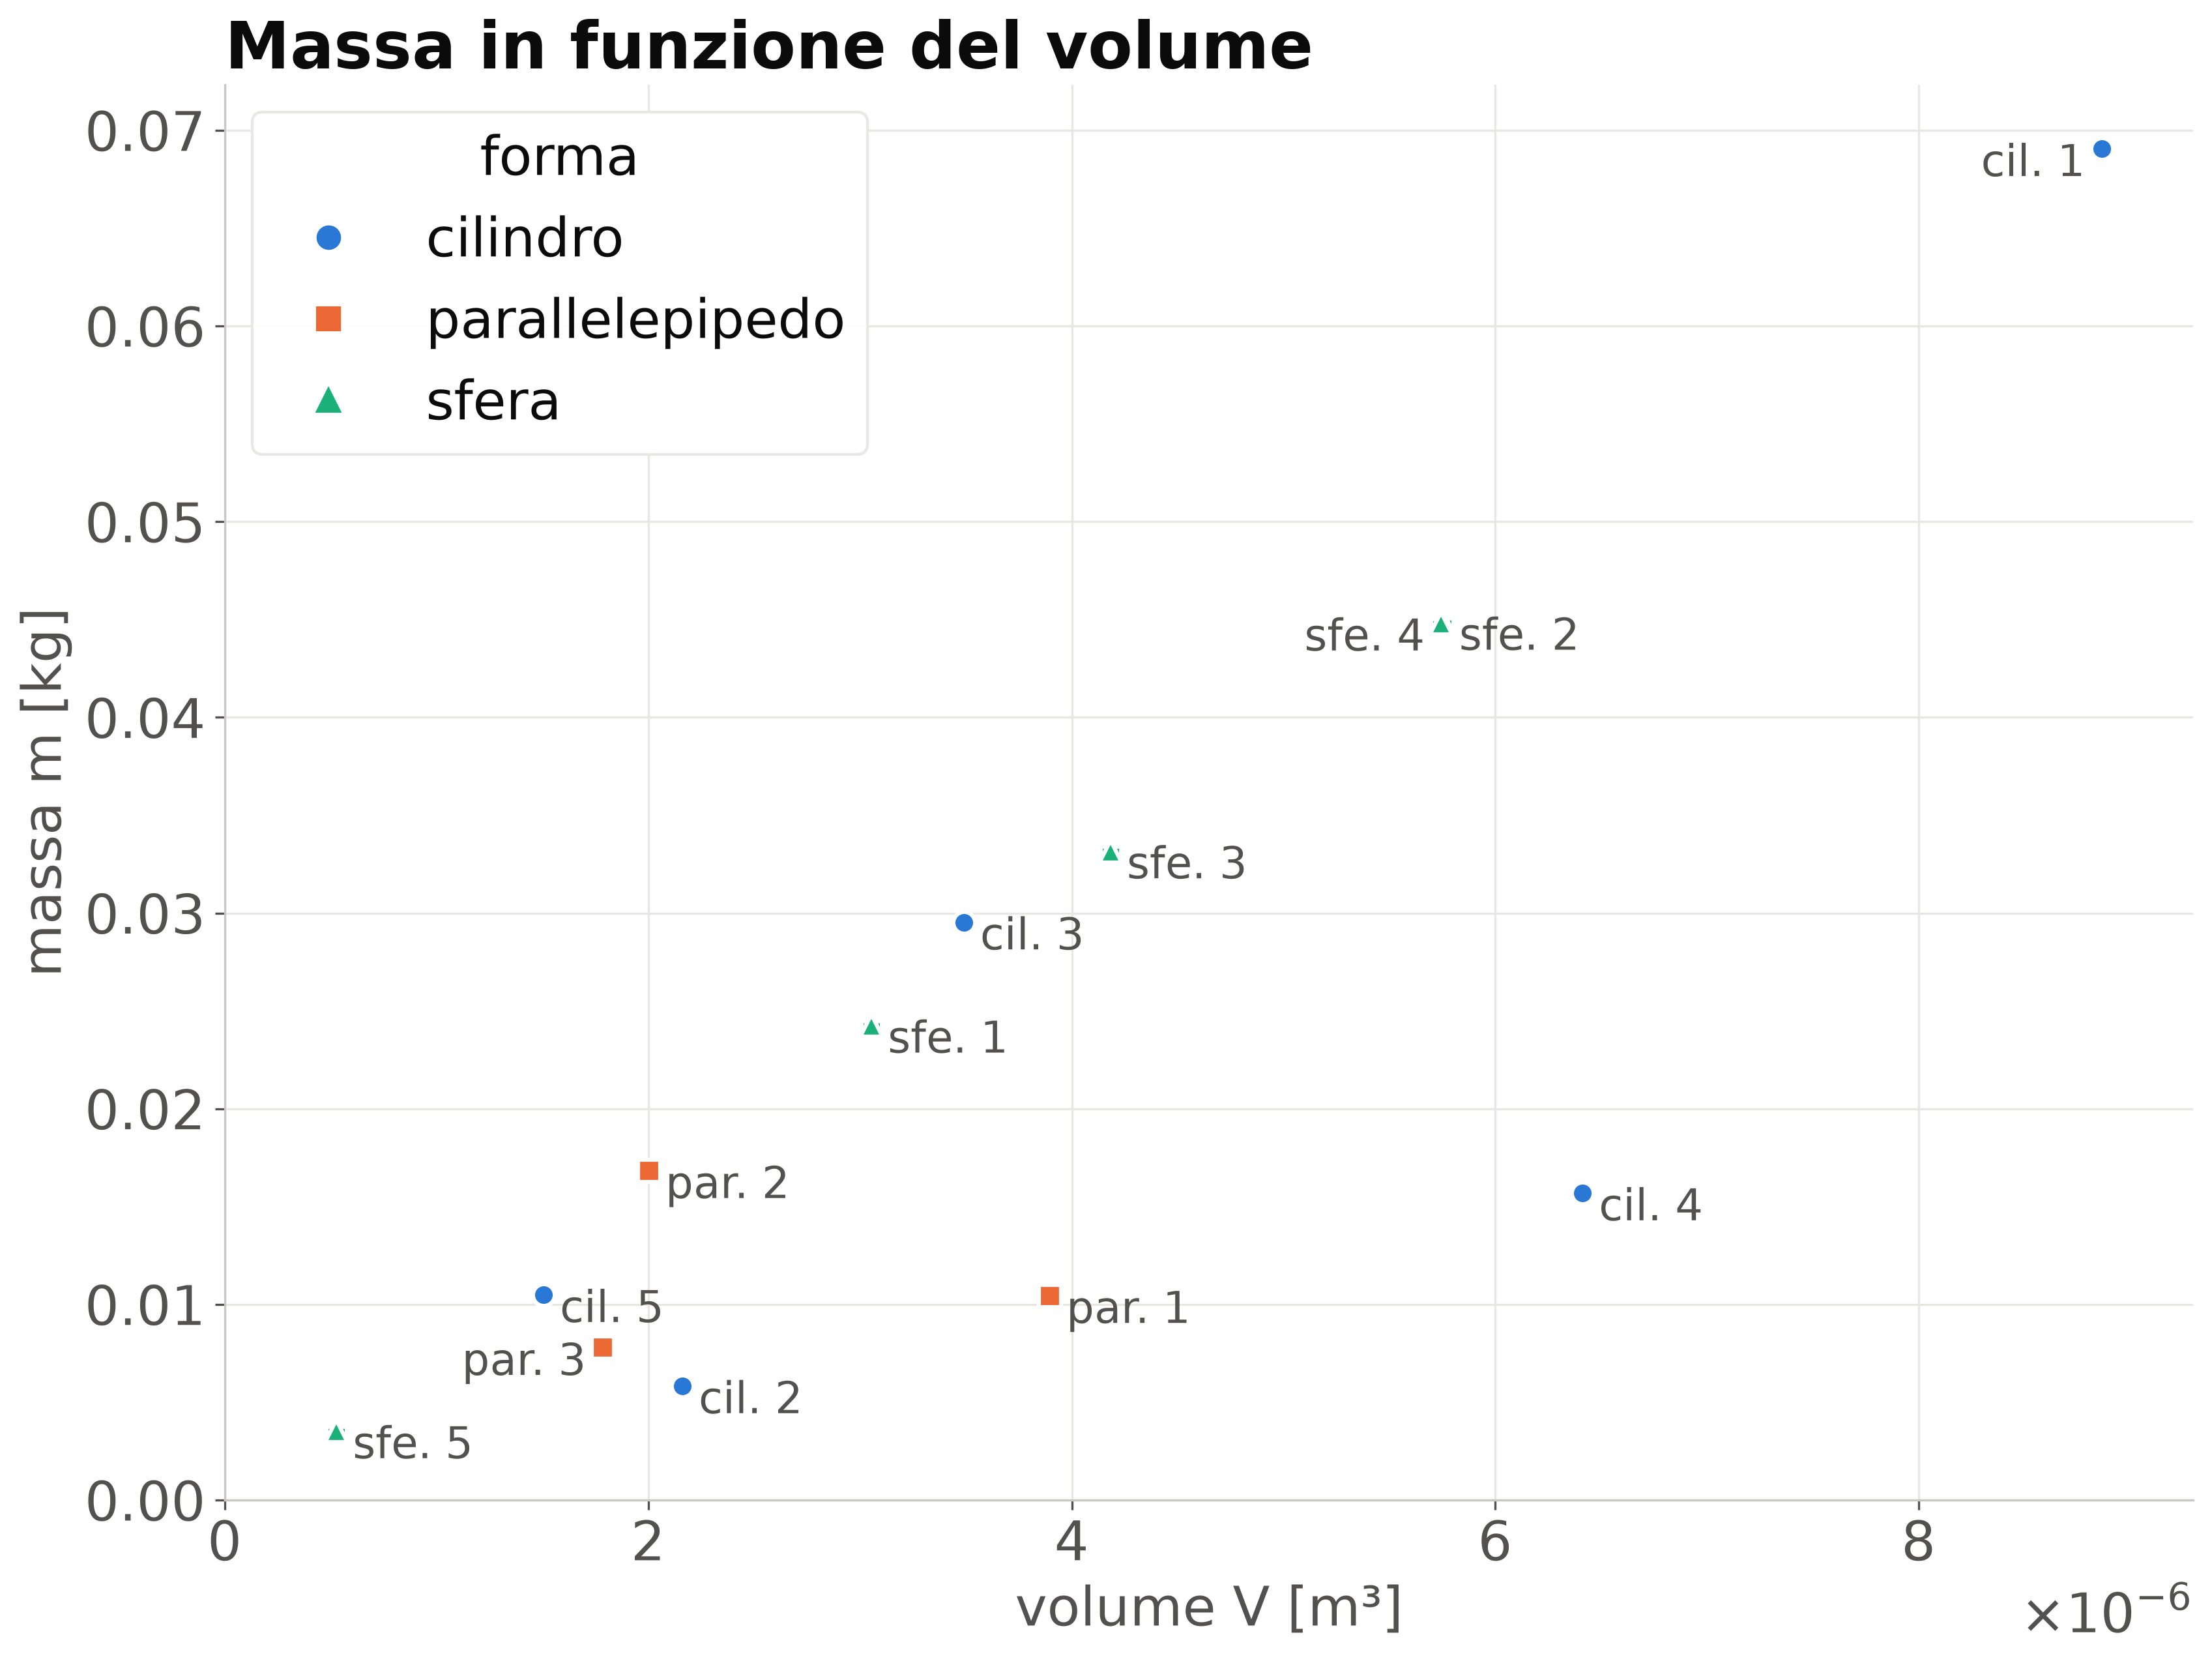
\includegraphics[width=\linewidth]{grafici/2_massa_e_volume.png}
    \caption{Volume in funzione della massa per tutti i solidi misurati.}
    \label{fig:massa_volume}
\end{figure}

Come possiamo vedere, le varie densità differiscono tra loro, ciò è dovuto al fatto che i materiali dei vari solidi sono diversi.

Dunque per classificare i vari materiali confrontiamo le densità con i valori tabulati. Presentiamo dunque una tabella dove sono riportati i valori tabulati dei materiali di cui possiamo assumere siano composti i solidi.

\begin{table}[htbp]
    \centering
    \begin{tabular}{c|c}
      materiale & $\rho$ (kg/m$^3$)\\
      \hline
        Alluminio & 2710 \\
        Acciaio inossidabile & 7480--8000 \\
        Ottone (lega Cu-Zn) & 8400--8700 \\
    \end{tabular}
    \caption{Densit\`a tabulate dei materiali con cui confrontare le misure}
    \label{tab:tabulati}
\end{table}

\newpage
\subsection{Classificazione del materiale dei solidi in base alla densità}

\begin{figure}[htbp]
    \centering
     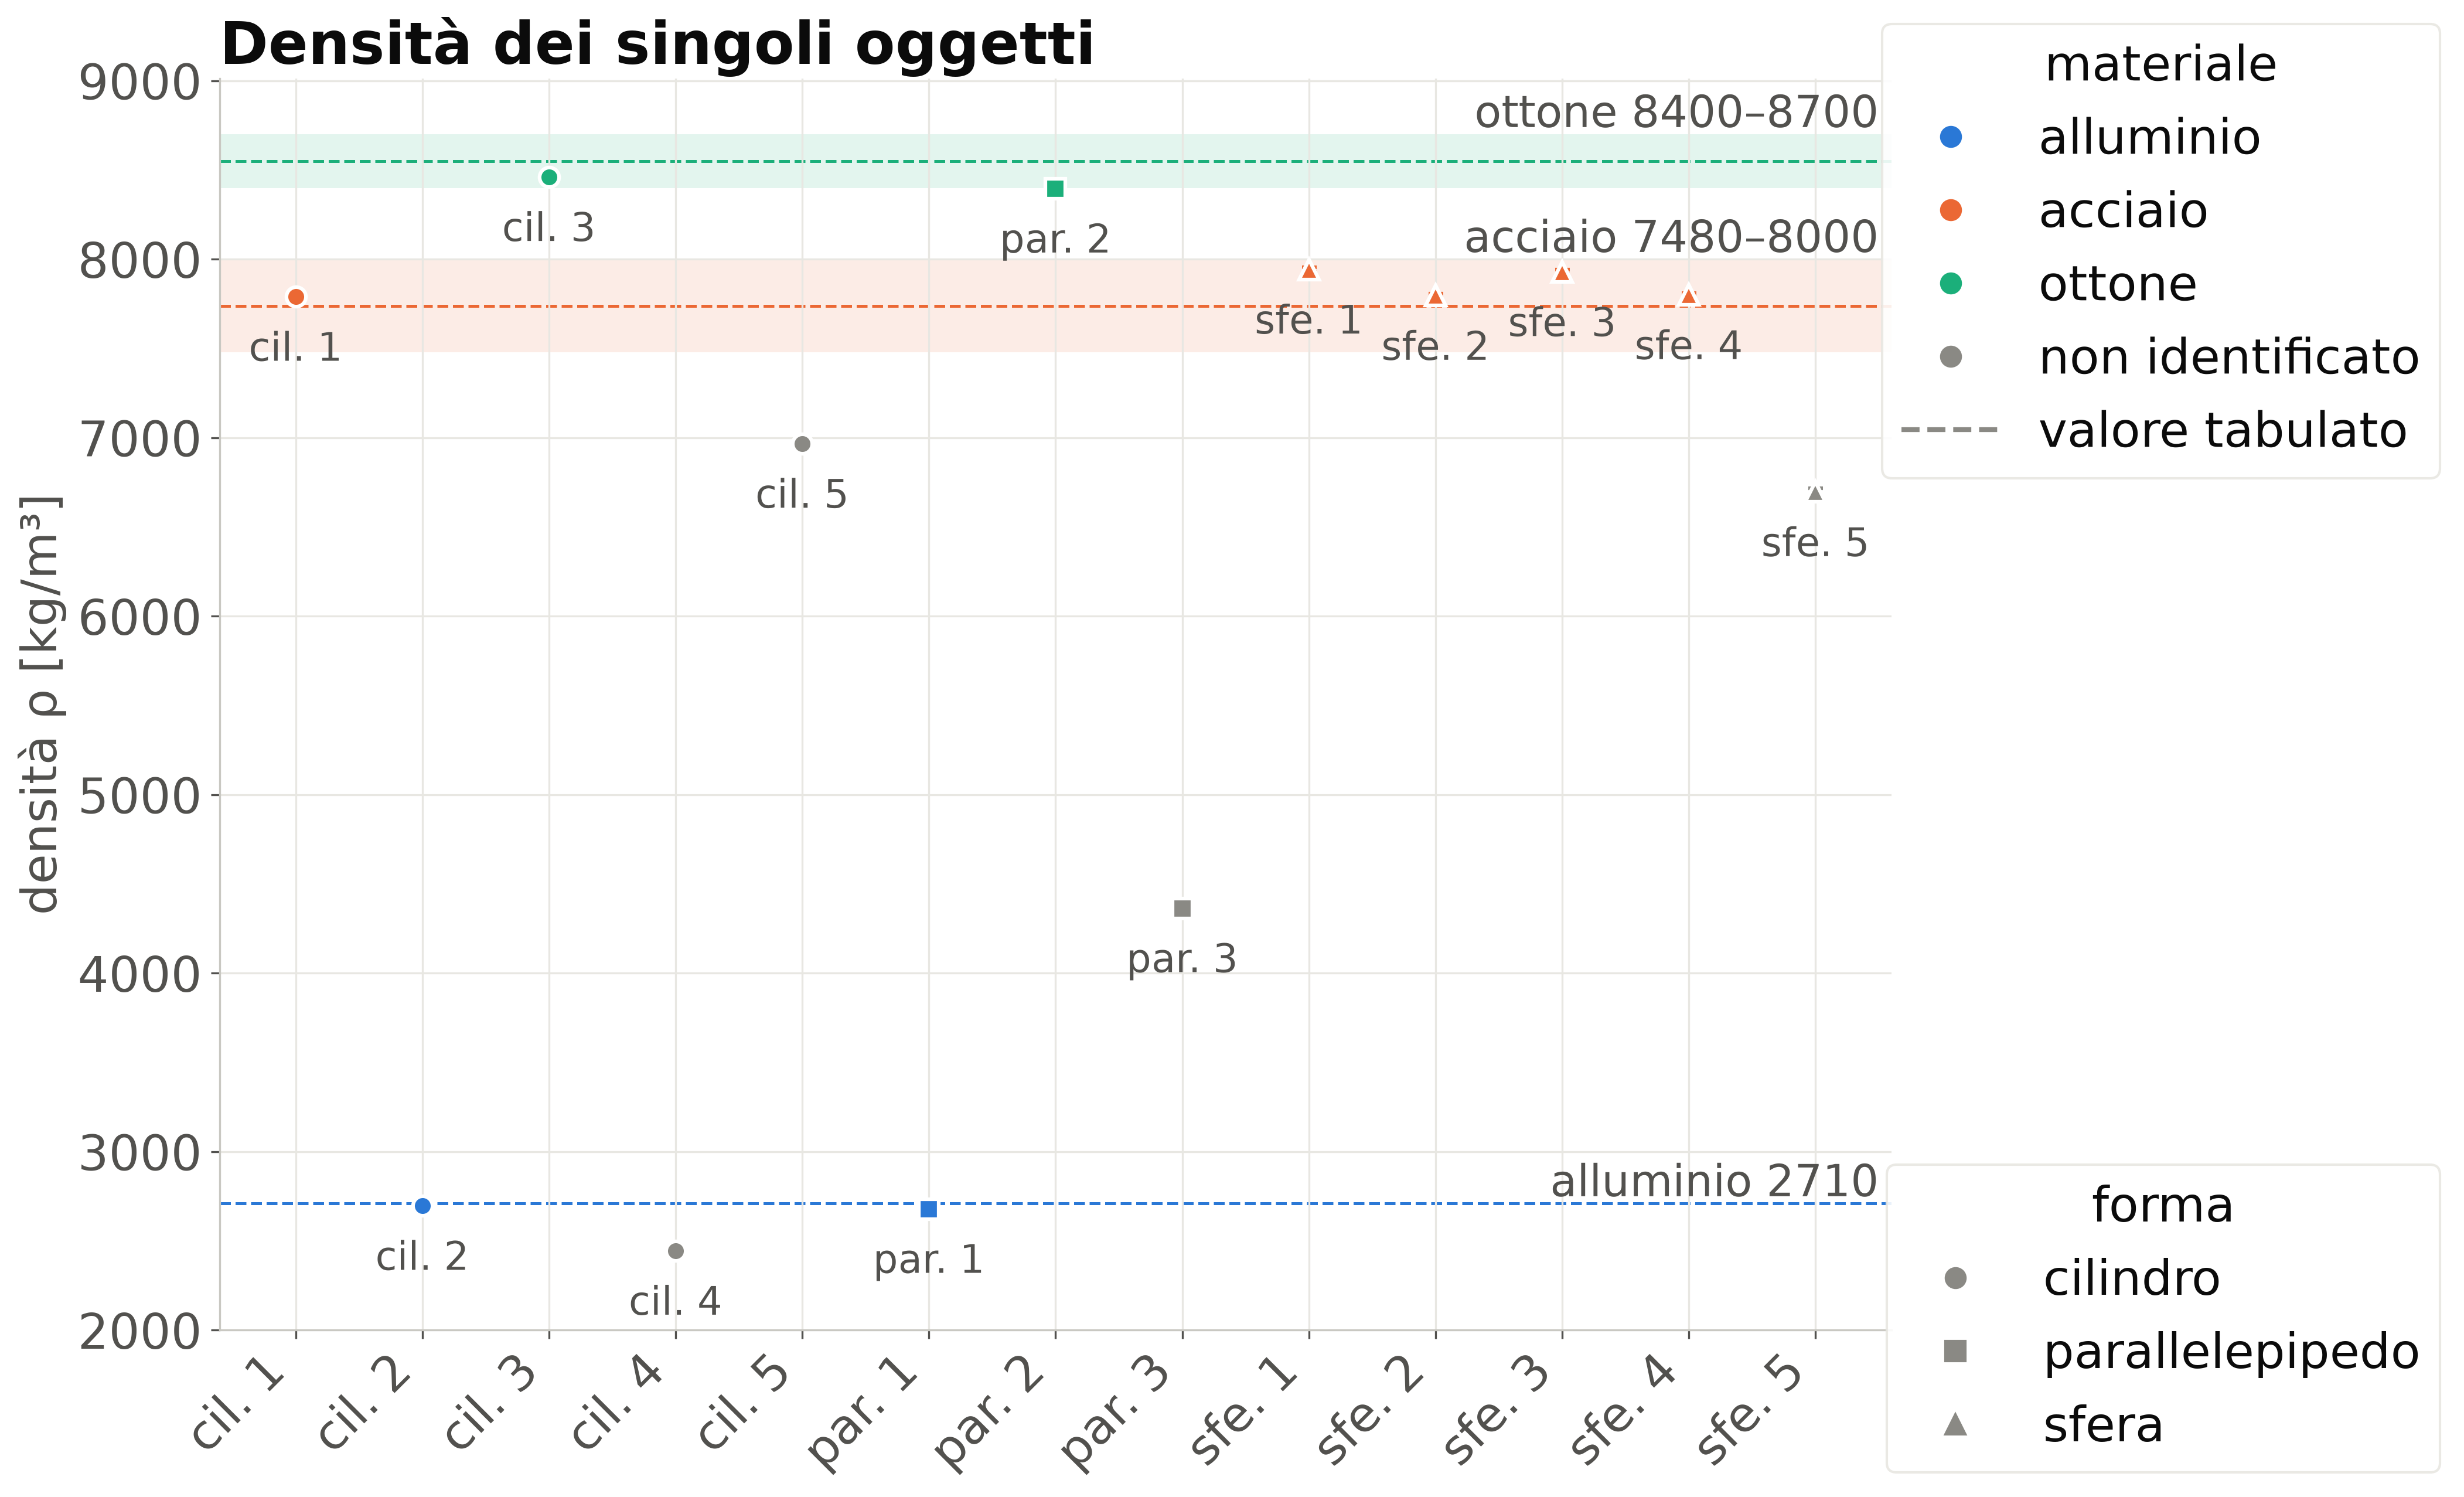
\includegraphics[width=\linewidth]{grafici/4a_densita_oggetti.png}
    \caption{Densità $\rho$ di ciascun solido. In ascissa è riportato l'identificativo del solido, in ordinata la densità. Le linee tratteggiate indicano i valori tabulati delle densità di alluminio, ottone e acciaio; le fasce colorate indicano gli intervalli di valori tabulati per le relative leghe.}
    \label{fig:densita_solidi}
\end{figure}

Il grafico in figura \ref{fig:densita_solidi} ci permette di riconoscere e classificare i materiali dei vari solidi basandoci sulla densità misurata.

Possiamo notare che alcuni solidi non corrispondono ad alcun materiale, stiamo trattando dei solidi: cilindro 5, sfera 5, parallelepipedo 3. \\ Le possibili cause per cui la densità di questi solidi non risulta compatibile con nessuno dei valori tabulati sono diverse: errori nelle misure dirette, irregolarità nella forma dei solidi (che rendono inadeguata la formula usata per il volume), oppure l'impiego di leghe di acciaio o ottone con composizione diversa da quella tabulata.

Sul luogo dell'esperienza avevamo classificato i materiali dei solidi visivamente basandoci principalmente sul colore. Di seguito la tabella con le nostre valutazioni.

\begin{table}[htbp]
    \centering
    \begin{tabular}{c|c|c}
        Solido & Materiale (visivo) & Scarto tra densità misurata e tabulata \\
        \hline
        Cilindro 5        & Ottone                & $-18\%$ \\
        Sfera 5           & Acciaio               & $-14\%$ \\
        Parallelepipedo 3 & Alluminio / Acciaio   & $+61\%$ / $-44\%$
    \end{tabular}
    \caption{Confronto tra la densità misurata dei solidi non identificati e la densità attesa per il materiale assegnato visivamente. Lo scarto è calcolato rispetto al valore centrale dell'intervallo della densità tabulata. Per il parallelepipedo 3 sono riportate entrambe le classificazioni possibili.}
    \label{tab:scarti_non_identificati}
\end{table}

Le possibili spiegazioni di queste discrepanze sono essenzialmente due: un errore nella determinazione del volume, oppure un materiale diverso da quello assegnato visivamente.

Un errore sulla massa è invece poco probabile. La massa, infatti, è stata misurata direttamente con una bilancia di risoluzione \SI{0.001}{g}, con un'incertezza relativa dell'ordine di $10^{-4}$, del tutto trascurabile rispetto agli scarti osservati; solo un errore sistematico evidente, come una bilancia non tarata, potrebbe giustificarli, ma in tal caso avrebbe interessato allo stesso modo anche gli altri solidi, che risultano invece compatibili con i valori tabulati.

Il volume, non essendo una misura diretta, è ricavato da più misure di lunghezza effettuate con il calibro, ciascuna soggetta a errori di lettura, e anche un piccolo errore su una dimensione si amplifica sul volume. Inoltre, il calcolo del volume presuppone un solido regolare, ipotesi non sempre verificata o prevedibile. È inoltre probabile che il volume sia sovrastimato, invece che sottostimato.

Per il cilindro 5 e la sfera 5 la densità misurata è inferiore a quella attesa, il che è compatibile sia con un volume sovrastimato perchè il calibro legge l’ingombro massimo, quindi smussi, bordi arrotondati e facce non parallele portano a sovrastimare il volume, sia con un materiale diverso, ad esempio una lega di composizione differente.

Il caso del parallelepipedo 3 è più incerto, poiché alluminio e acciaio, essendo entrambi grigi, sono difficili da distinguere a vista. Se fosse di acciaio, la densità sarebbe inferiore del 44\% a quella attesa: uno scarto troppo grande per un semplice errore di lettura, che suggerirebbe piuttosto la presenza di una cavità o un grande errore nella misura di una delle dimensioni. Se invece fosse di alluminio, la densità risulterebbe superiore del 61\% a quella attesa: in questo caso cavità o irregolarità sono da escludere, e restano come spiegazioni un volume sottostimato per un errore di misurazione, oppure un materiale diverso, più denso dell'alluminio ma di aspetto simile come ad esempio il titanio con una densità tabulata di 4507 kg/m$^3$.


Per questi motivi, i tre solidi sono stati esclusi dai fit lineari descritti nella sezione successiva. Abbiamo deciso di escludere anche il cilindro 4, che ha una densità ($2446.5 \pm 2.7$~kg/m$^3$) vicina a quella dell'alluminio ma più bassa di circa il 10\%. Questo solido infatti è l'unico che è risultato irregolare secondo il criterio che abbiamo usato nelle misure dirette, quindi la formula del volume non è affidabile per lui.

\subsection{Determinazione della densità tramite fit lineare}\label{sec:fit}

Come detto nei cenni teorici, per corpi dello stesso materiale il volume è proporzionale alla massa. Per ogni materiale abbiamo quindi fatto un fit lineare del volume in funzione della massa,
\begin{equation}
    V = \alpha\, m + \beta,
    \label{eq:fit}
\end{equation}
usando come incertezze sulle ordinate le $\sigma_V$ che abbiamo calcolato con la propagazione. Le incertezze sulla massa le abbiamo trascurate, perché la loro incertezza relativa ($\sim 10^{-4}$) è molto più piccola di quella sul volume. Dalla \eqref{eq:densita} ci aspettiamo $\beta \simeq 0$ e $\alpha = 1/\rho$, quindi la densità e la sua incertezza si ricavano come
\begin{equation}
    \rho = \frac{1}{\alpha}, \qquad \sigma_\rho = \frac{\sigma_\alpha}{\alpha^2}.
    \label{eq:rho_fit}
\end{equation}
Siccome $V$ è in mm$^3$ e $m$ in g, $\alpha$ è in mm$^3$/g e quindi $1/\alpha$ è in g/mm$^3$; per avere la densità in kg/m$^3$ bisogna moltiplicare per $10^6$.

I solidi sono stati divisi per materiale in base alla classificazione fatta nella sezione precedente:
\begin{itemize}
    \item alluminio: cilindro 2 e parallelepipedo 1;
    \item ottone: cilindro 3 e parallelepipedo 2;
    \item acciaio: cilindro 1 e sfere 1--4.
\end{itemize}
In figura \ref{fig:fit_tutti} sono riportati i tre fit insieme, mentre in tabella \ref{tab:fit} riportiamo i parametri ottenuti.

\begin{figure}[htbp]
    \centering
    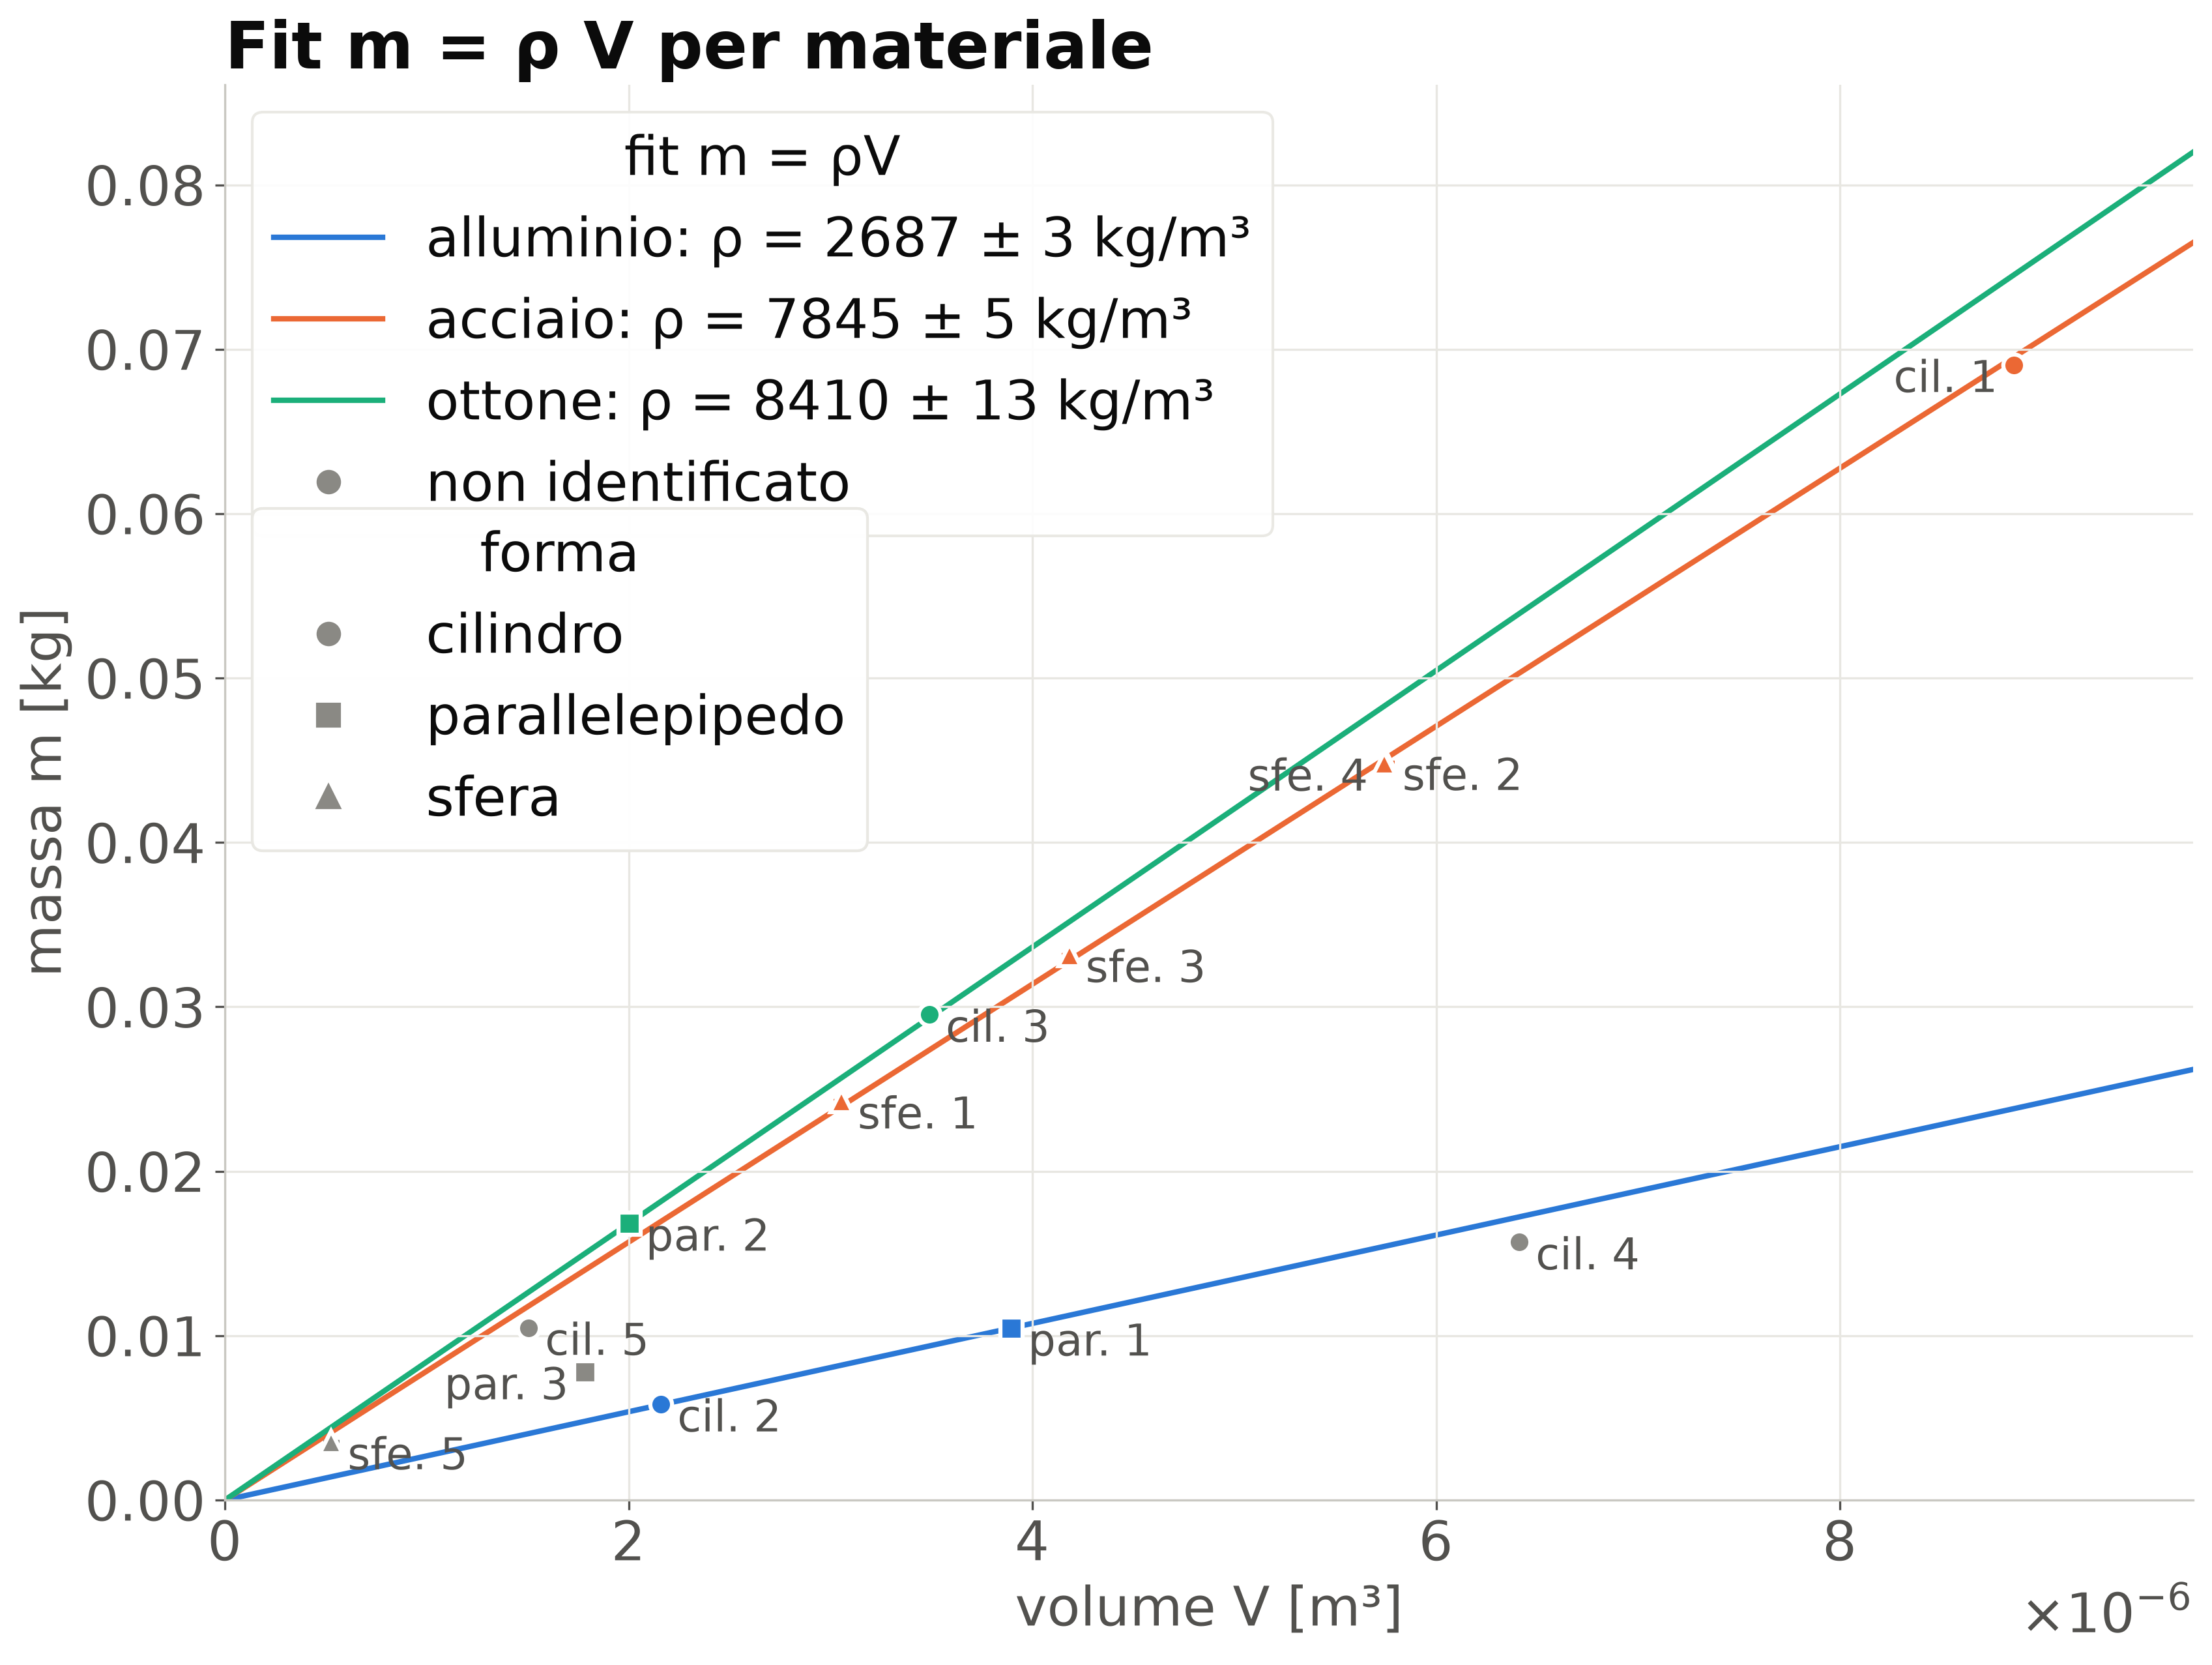
\includegraphics[width=\linewidth]{grafici/3_fit_densita.png}
    \caption{Fit lineari $V = \alpha m + \beta$ per i tre materiali.}
    \label{fig:fit_tutti}
\end{figure}

\begin{table}[htbp]
    \centering
    \begin{tabular}{c|c|c|c|c}
      materiale & $\alpha\pm\sigma_\alpha$ (mm$^3$/g) & $\beta\pm\sigma_\beta$ (mm$^3$) & $\rho\pm\sigma_\rho$ (kg/m$^3$) & $\rho_{\text{tab}}$ (kg/m$^3$)\\
      \hline
      Alluminio & $376.2 \pm 1.3$ & $-32 \pm 11$ & $2658 \pm 10$ & 2710 \\
      Ottone    & $117.18 \pm 0.97$ & $33 \pm 17$ & $8534 \pm 71$ & 8400--8700 \\
      Acciaio   & $130.30 \pm 0.24$ & $-112.0 \pm 9.3$ & $7675 \pm 14$ & 7480--8000 \\
    \end{tabular}
    \caption{Parametri dei fit lineari $V = \alpha m + \beta$ e densit\`a ricavate con la \eqref{eq:rho_fit}, confrontate con i valori tabulati.}
    \label{tab:fit}
\end{table}

\subsubsection*{Acciaio}

\begin{figure}[htbp]
    \centering
    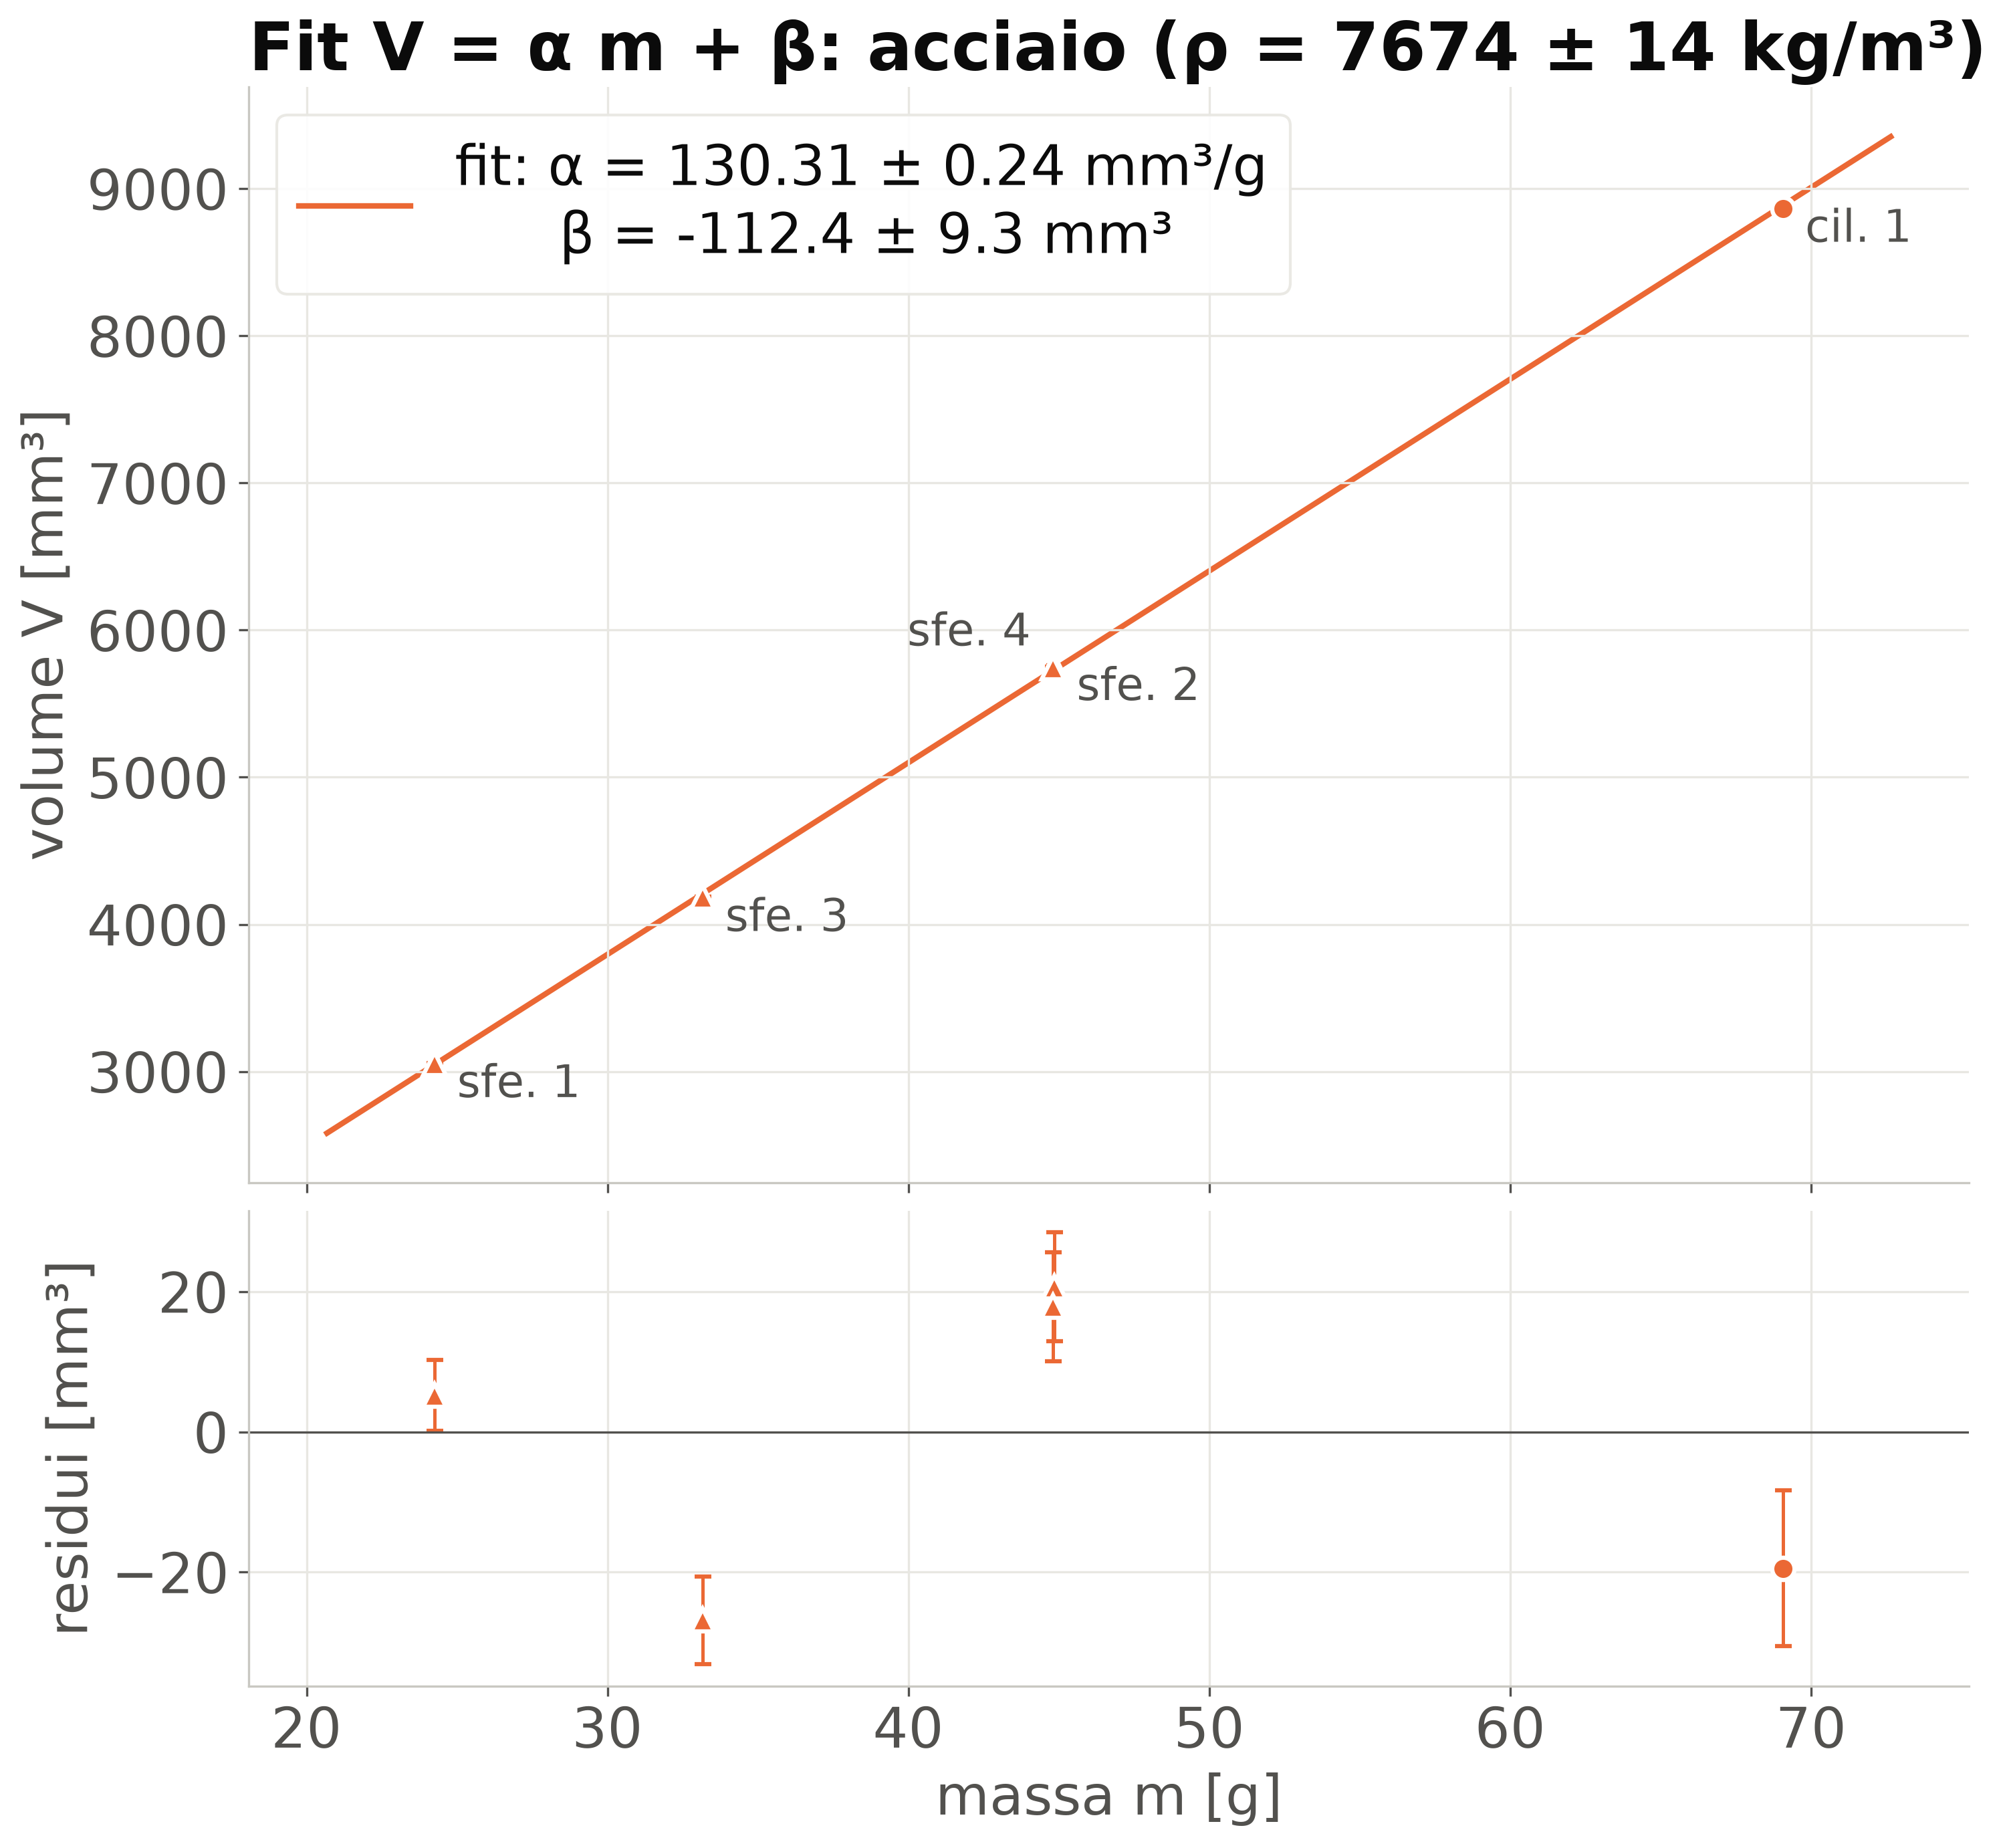
\includegraphics[width=0.75\linewidth]{grafici/b_fit_acciaio.png}
    \caption{Fit lineare $V = \alpha m + \beta$ per i solidi in acciaio.}
    \label{fig:fit_acciaio}
\end{figure}

Dal fit sui solidi in acciaio (figura \ref{fig:fit_acciaio}) otteniamo $\rho = 7675 \pm 14$~kg/m$^3$, che è compatibile con l'intervallo tabulato 7480--8000~kg/m$^3$. L'intercetta invece vale $\beta = -112.0 \pm 9.3$~mm$^3$, che dista circa $12\,\sigma_\beta$ da zero, quindi la retta non passa per l'origine come ci aspettavamo. Notiamo anche che la densità del fit è più bassa di quelle di tutti i singoli solidi (che vanno da 7788 a 7943~kg/m$^3$): questo succede perché una parte dell'andamento dei dati finisce nell'intercetta invece che nella pendenza.

\begin{figure}[htbp]
    \centering
    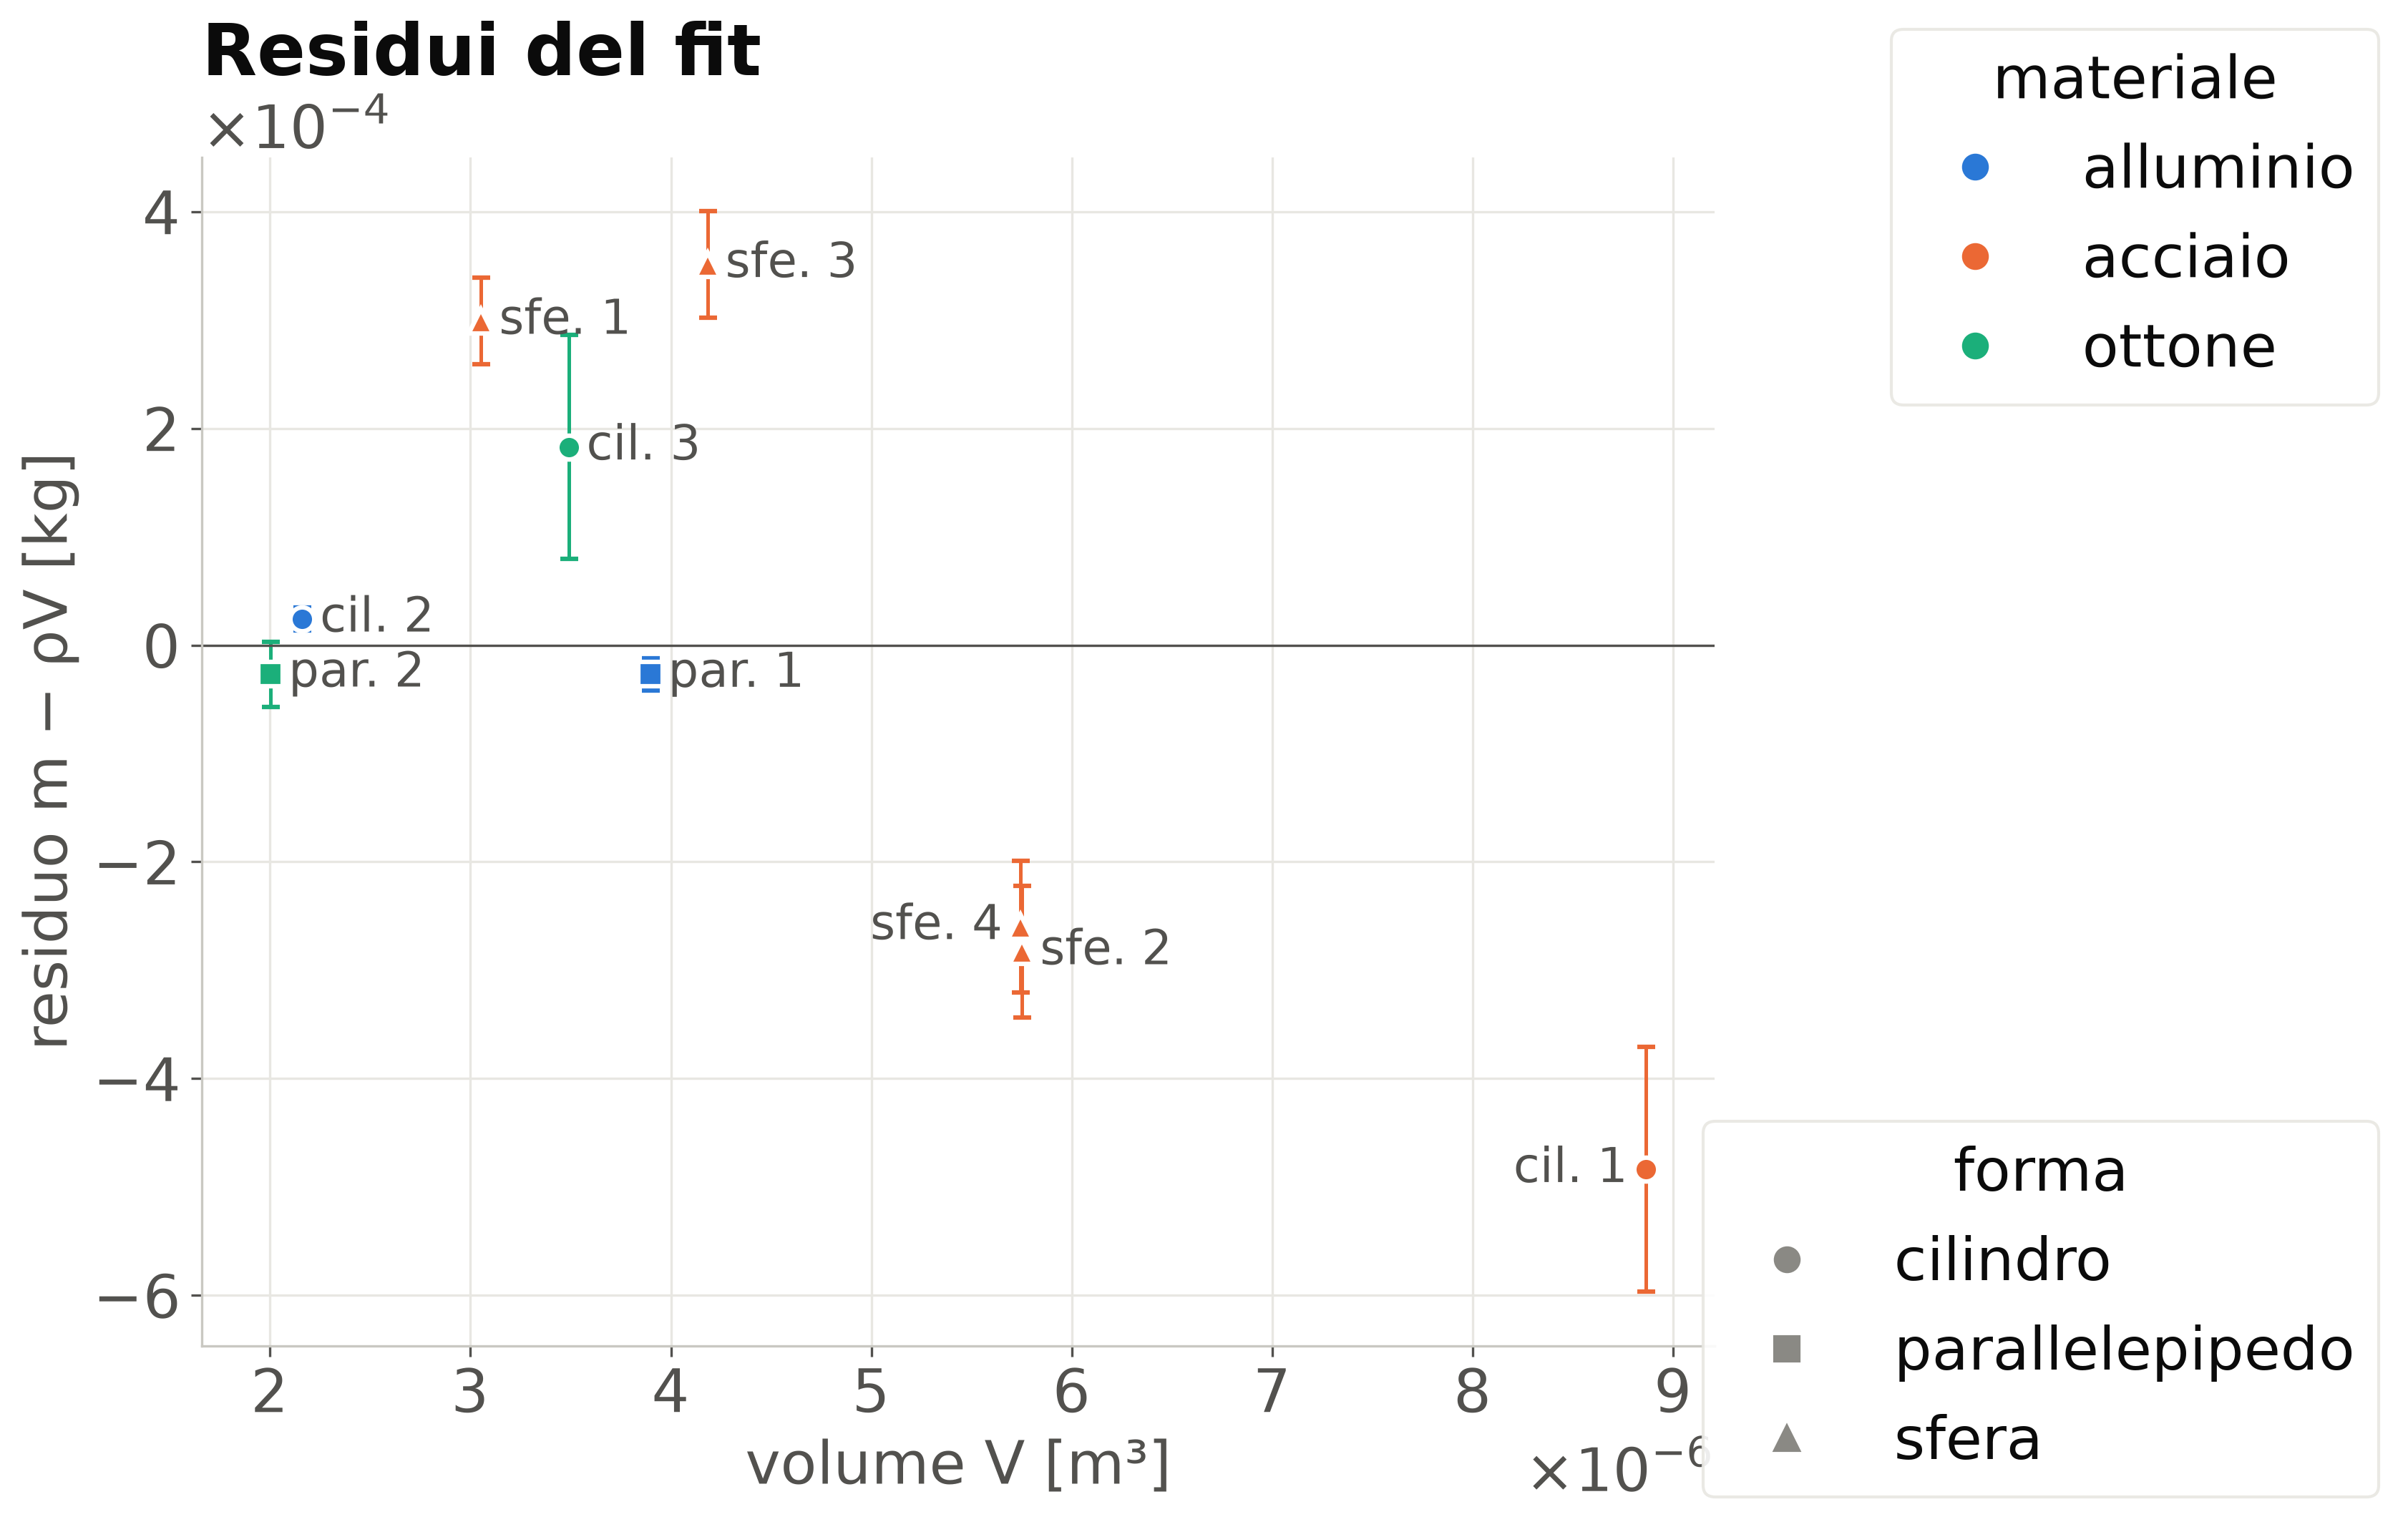
\includegraphics[width=\linewidth]{grafici/5_residui.png}
    \caption{Residui dei fit lineari.}
    \label{fig:residui}
\end{figure}

Nel grafico dei residui (figura \ref{fig:residui}) si vede che alcuni punti dell'acciaio escono dalle barre d'errore, la sfera 3 ad esempio è a circa $4\,\sigma$ dalla retta, quindi la retta non descrive i punti entro le loro incertezze.

Secondo noi le cause sono due. La prima è che le barre d'errore sul volume tengono conto solo della risoluzione degli strumenti, quindi sono probabilmente sottostimate, perché non considerano le piccole imperfezioni della forma dei solidi. La seconda, più importante, è che i solidi probabilmente non sono tutti fatti dello stesso acciaio. Guardando la tabella \ref{tab:mVr_sfere} infatti si vede che le sfere 1 e 3 hanno densità intorno a 7930--7940~kg/m$^3$, mentre le sfere 2 e 4 e il cilindro 1 stanno intorno a 7790--7800~kg/m$^3$. La differenza è di circa 140~kg/m$^3$, più di dieci volte le incertezze, quindi non può essere un errore di misura e fa pensare a due acciai con composizione un po' diversa. Siccome le sfere più leggere (1 e 3) sono anche le più dense, i punti non riescono a stare tutti su una retta che passa per l'origine, e il fit "compensa" con un'intercetta negativa. Per questo la densità che otteniamo dal fit è una specie di media tra i due acciai e non la densità di uno solo.

\subsubsection*{Alluminio e ottone}

\begin{figure}[htbp]
    \centering
    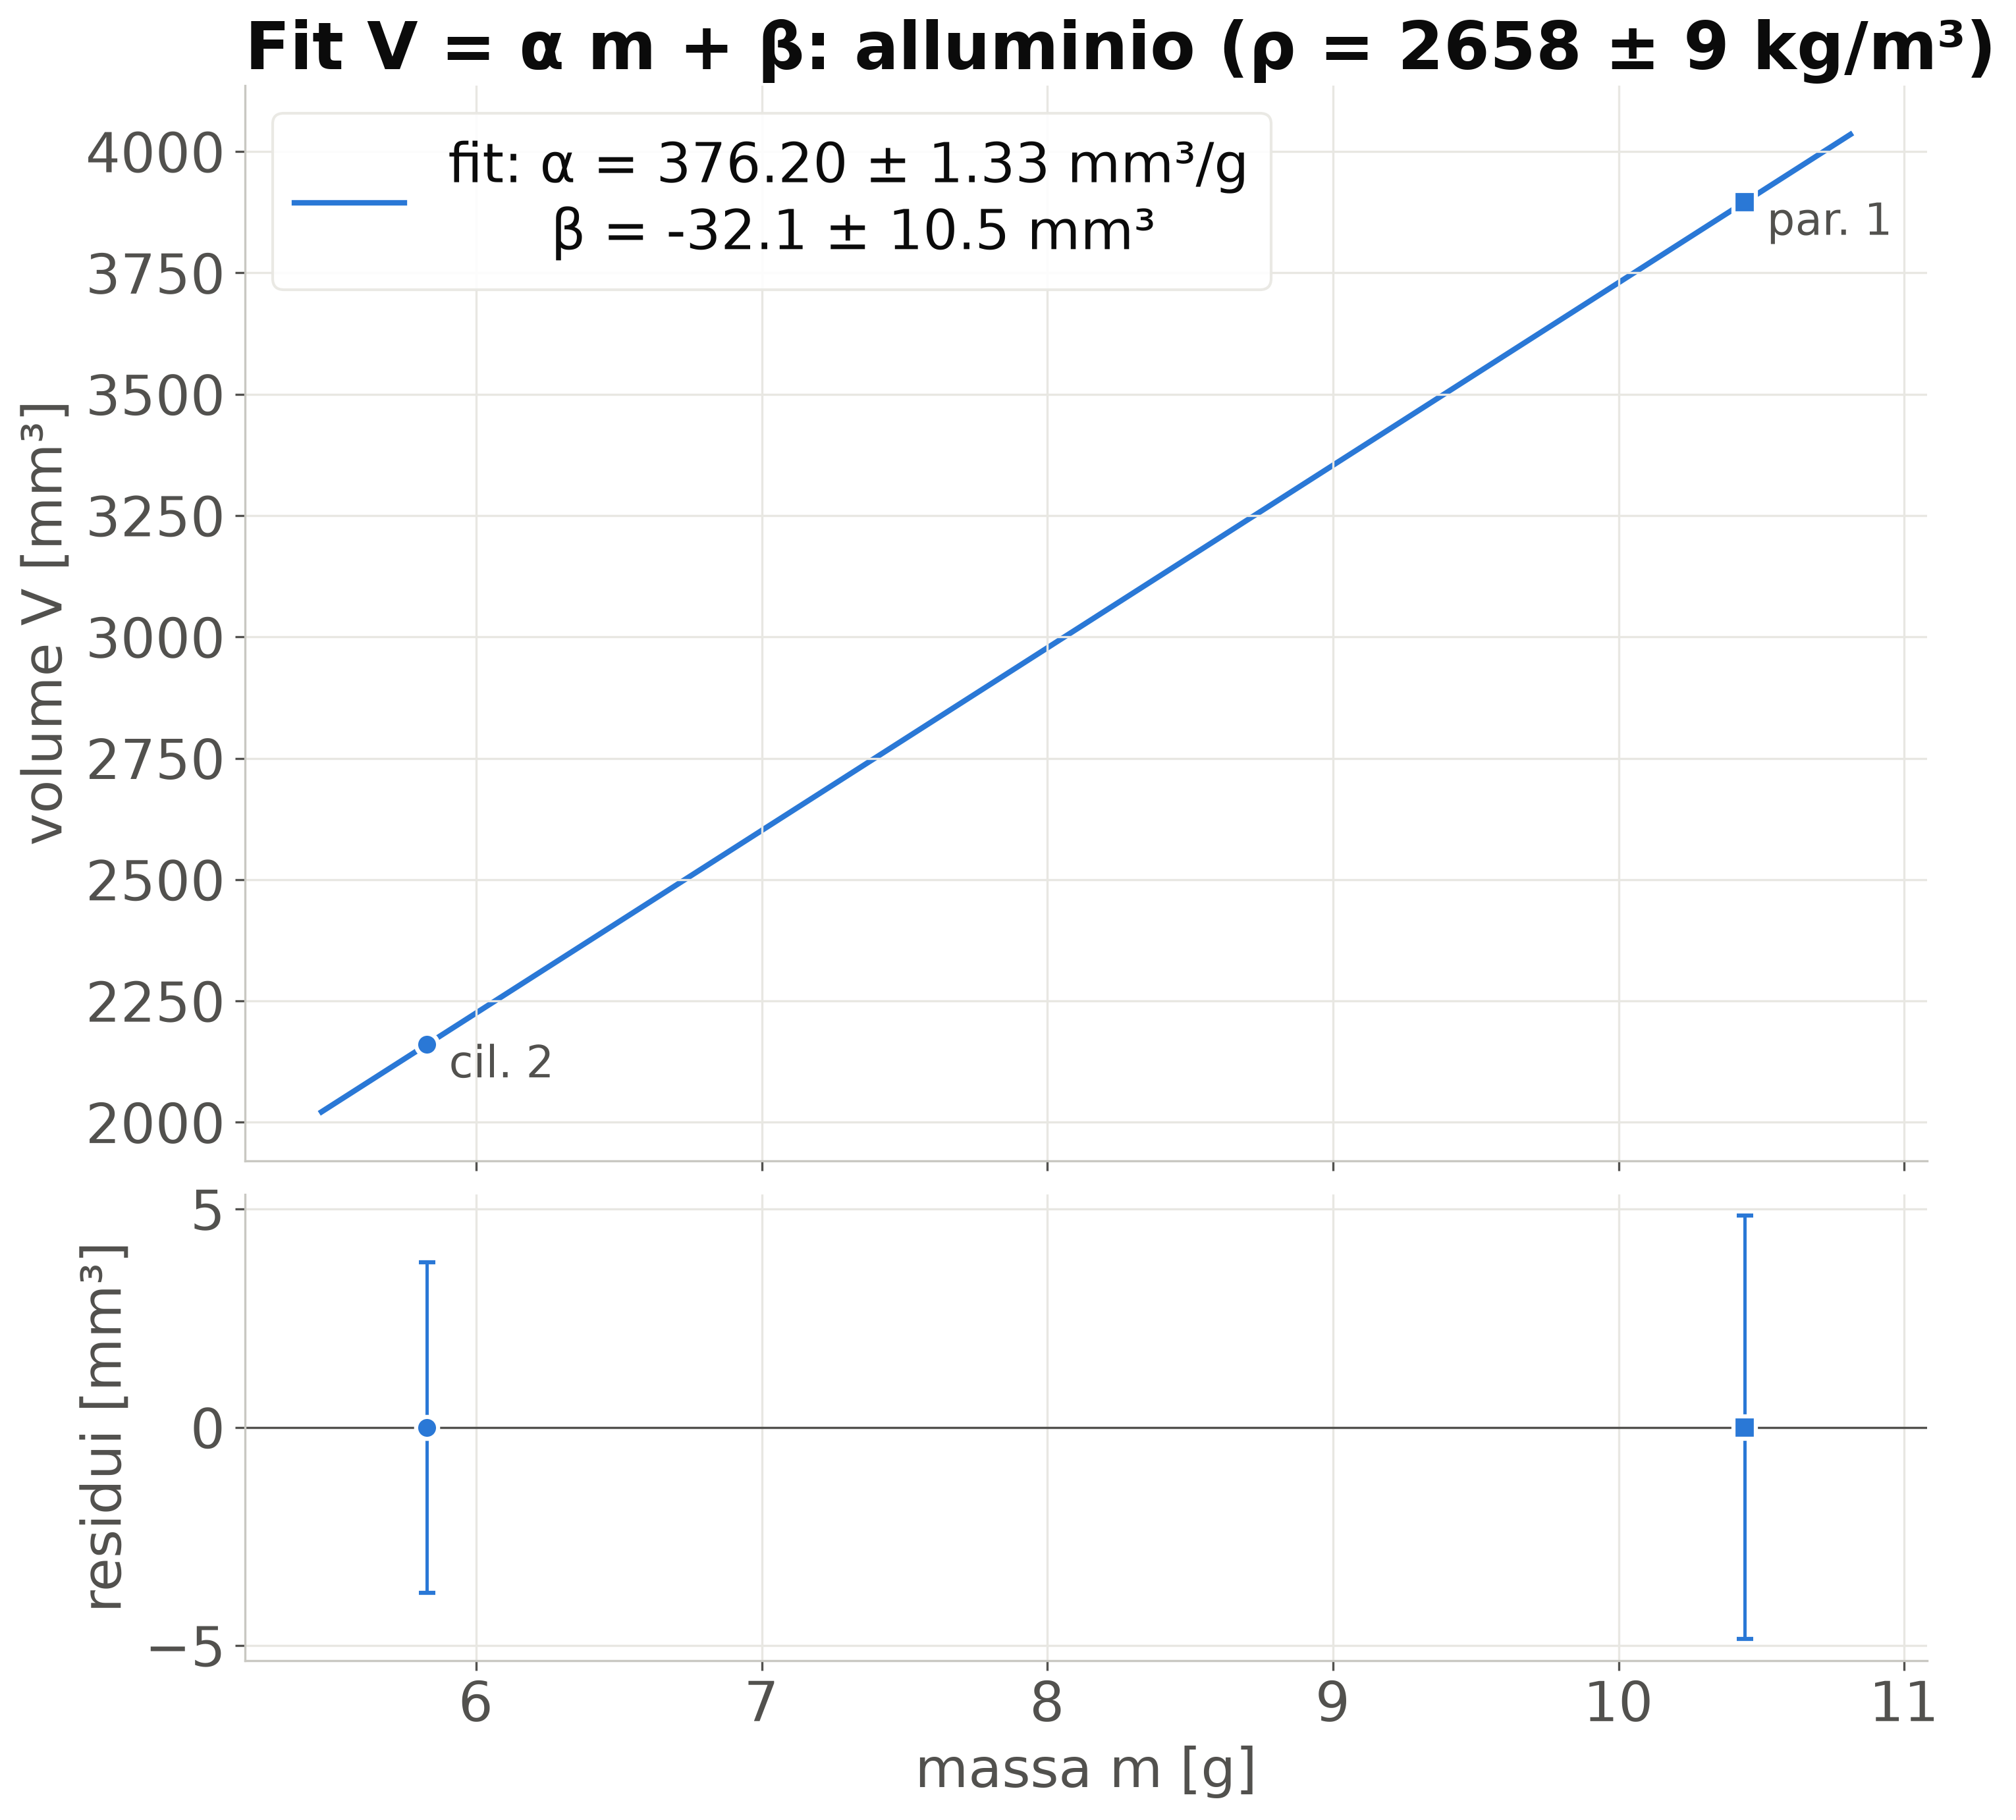
\includegraphics[width=0.75\linewidth]{grafici/b_fit_alluminio.png}
    \caption{Fit lineare $V = \alpha m + \beta$ per i solidi in alluminio.}
    \label{fig:fit_alluminio}
\end{figure}

\begin{figure}[htbp]
    \centering
    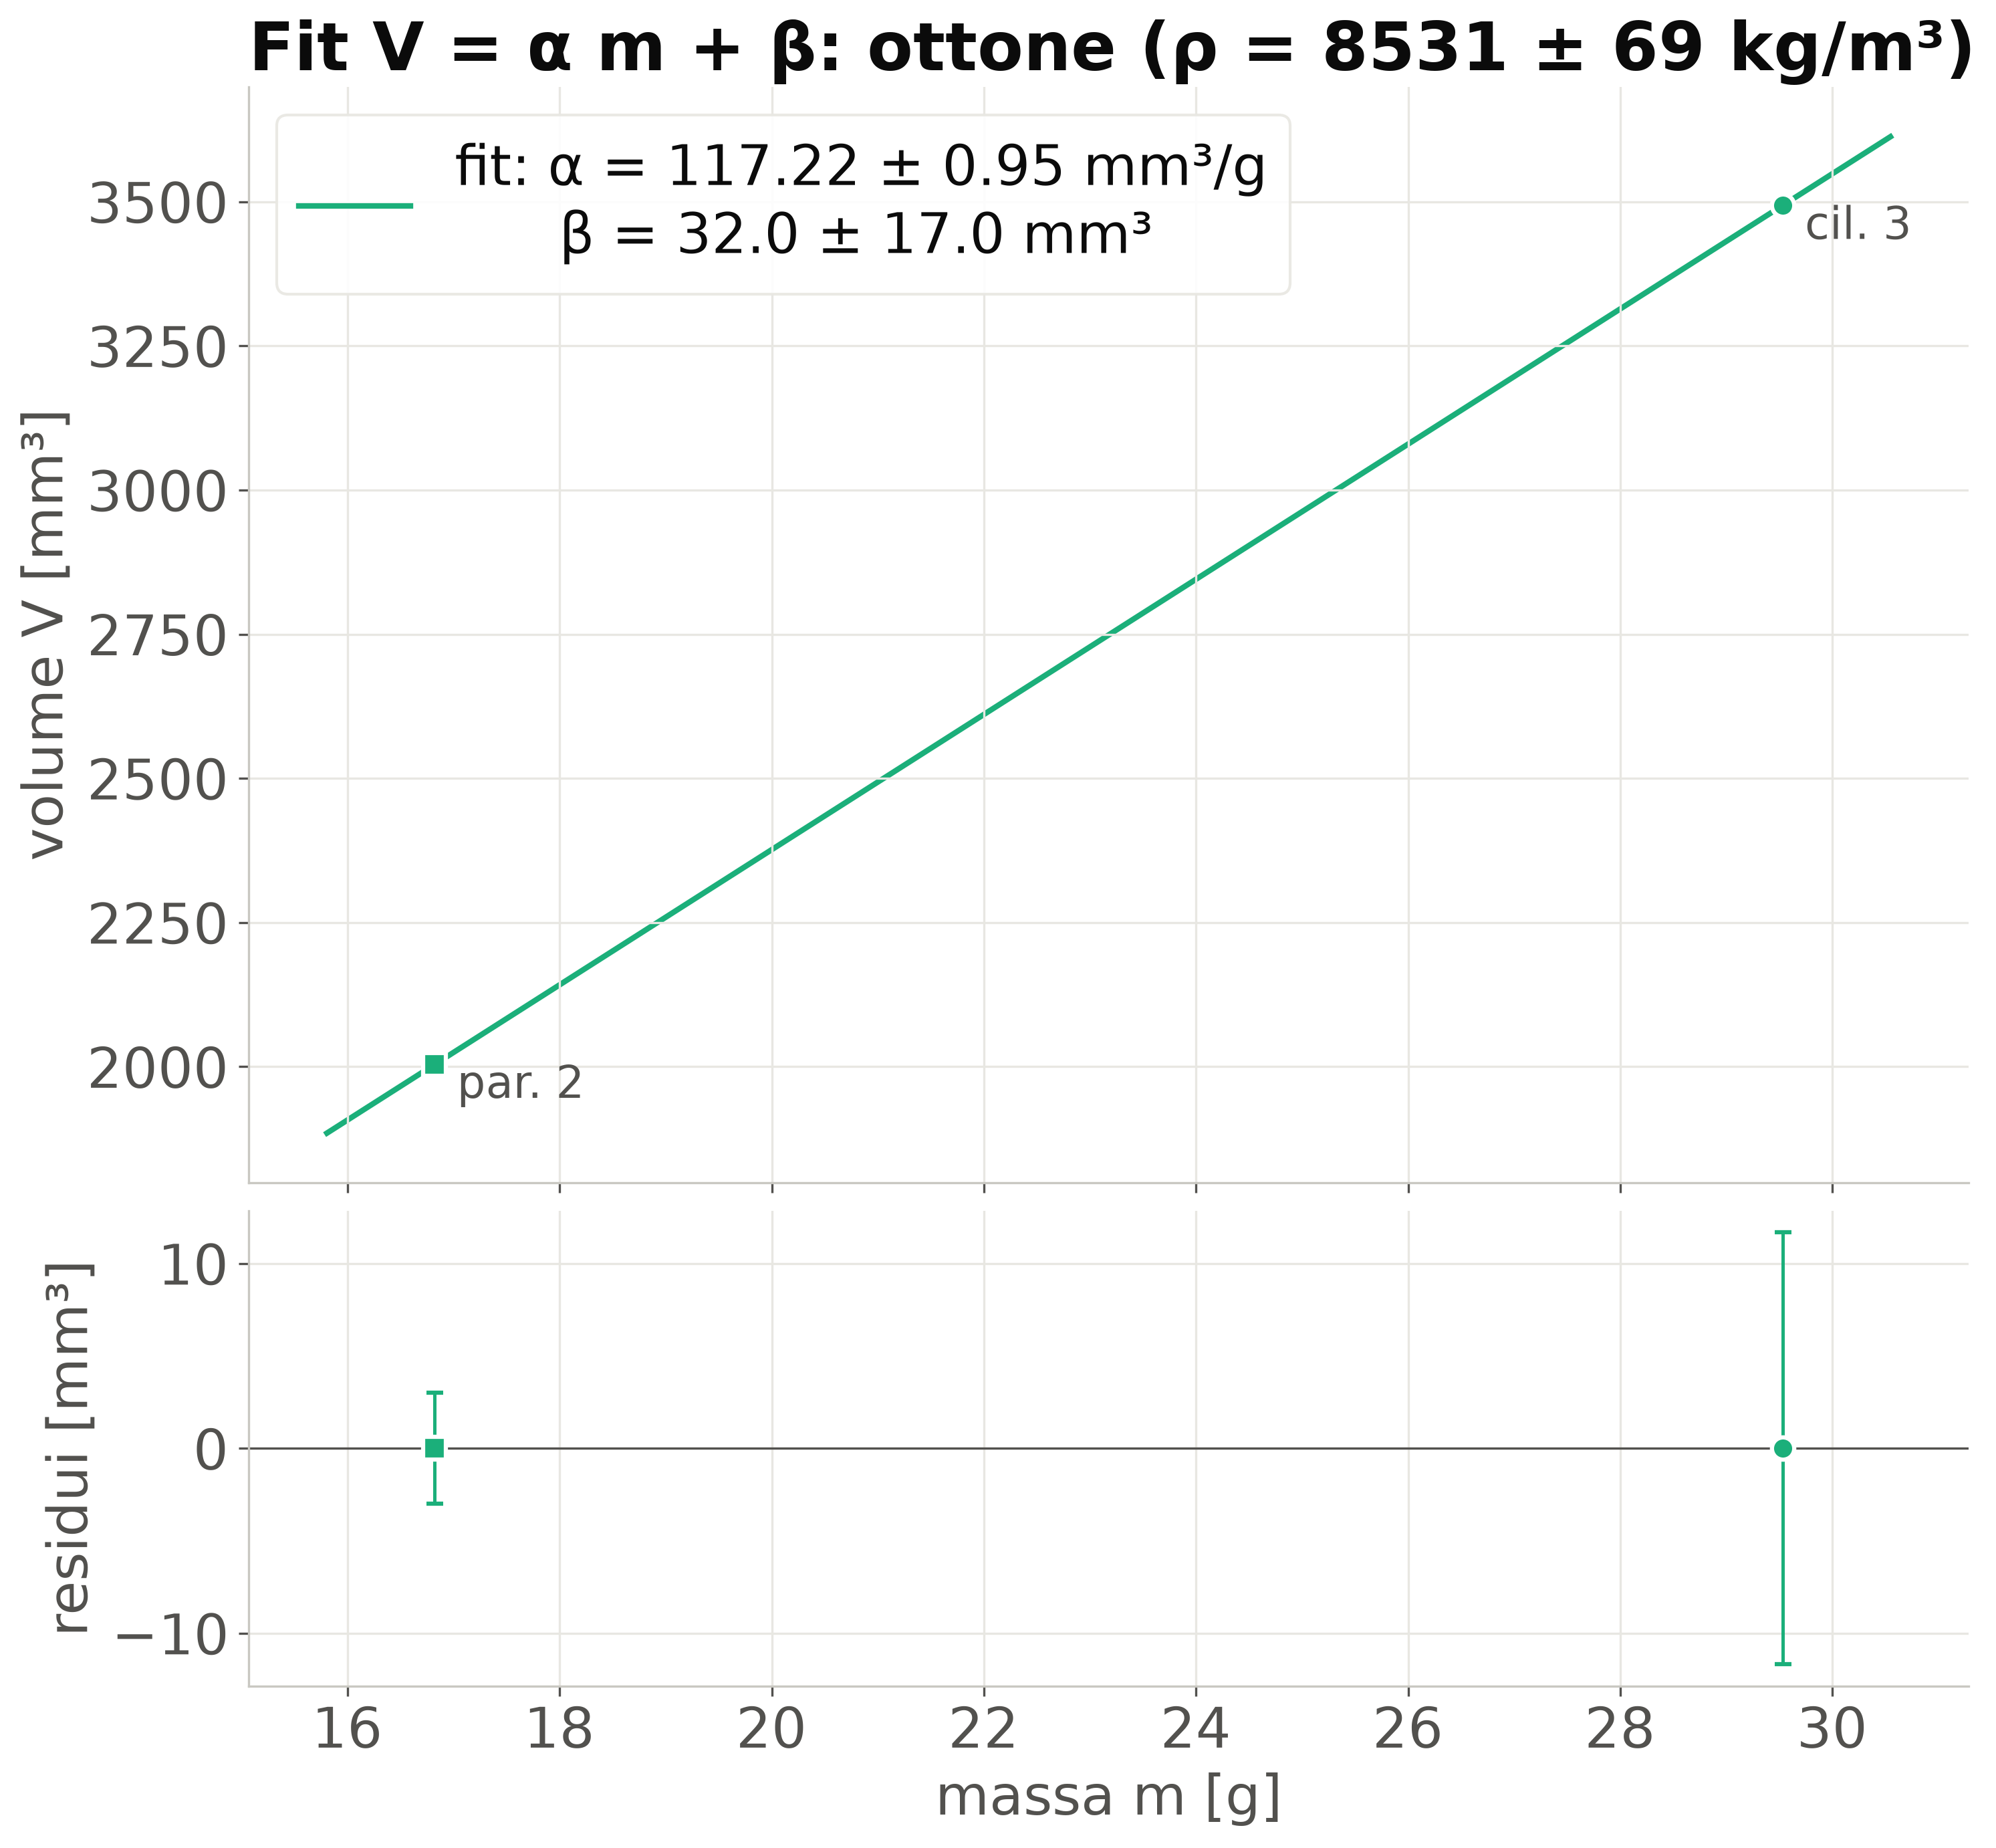
\includegraphics[width=0.75\linewidth]{grafici/b_fit_ottone.png}
    \caption{Fit lineare $V = \alpha m + \beta$ per i solidi in ottone.}
    \label{fig:fit_ottone}
\end{figure}

Per l'alluminio (figura \ref{fig:fit_alluminio}) e per l'ottone (figura \ref{fig:fit_ottone}) invece abbiamo solo due punti ciascuno. Una retta per due punti passa sempre esattamente per entrambi, quindi i residui sono zero per forza e non ci dicono niente sulla bontà del fit; allo stesso modo non possiamo verificare se i punti siano davvero allineati su una retta che passa per l'origine. L'incertezza su $\alpha$ in questo caso viene solo dalle barre d'errore dei due punti.

Tenendo conto di questo, per l'ottone otteniamo $\rho = 8534 \pm 71$~kg/m$^3$, che è compatibile con l'intervallo tabulato 8400--8700~kg/m$^3$, e l'intercetta $\beta = 33 \pm 17$~mm$^3$ è compatibile con zero entro $2\,\sigma_\beta$.

Per l'alluminio invece otteniamo $\rho = 2658 \pm 10$~kg/m$^3$. Rispetto al valore tabulato la differenza è di 52~kg/m$^3$, cioè circa il 2\%, ma siccome l'incertezza è piccola questo corrisponde a circa $5\,\sigma_\rho$, quindi il valore non è compatibile con 2710~kg/m$^3$. Lo scarto però è piccolo e potrebbe essere dovuto al fatto che i solidi sono fatti di una lega di alluminio e non di alluminio puro. L'intercetta vale $\beta = -32 \pm 11$~mm$^3$, cioè circa $3\,\sigma_\beta$ da zero: questo succede perché i due solidi non hanno esattamente la stessa densità (2698 e 2680~kg/m$^3$), e con solo due punti questa differenza si vede subito nell'intercetta.

\subsection{Legge di scala $m = k r^3$ per le sfere}\label{sec:bilog}

Per una sfera omogenea vale $m = \rho \cdot \frac{4}{3}\pi r^3$, cioè $m = k r^3$ con $k = \frac{4}{3}\pi\rho$. Facendo il logaritmo di entrambi i membri otteniamo una relazione lineare:
\begin{equation}
    \ln m = \ln k + n \ln r,
    \label{eq:bilog}
\end{equation}
dove ci aspettiamo che la pendenza sia $n = 3$. Abbiamo quindi fatto un fit lineare di $\ln m$ in funzione di $\ln r$, con $r = d/2$, usando le sfere 1--4. La sfera 5 non l'abbiamo usata, perché la sua densità è diversa da quella delle altre e la \eqref{eq:bilog} funziona solo se le sfere sono tutte dello stesso materiale, cioè hanno lo stesso $k$.

Le incertezze sui logaritmi si ottengono come $\sigma_{\ln r} = \sigma_r / r$ e $\sigma_{\ln m} = \sigma_m / m$, con $\sigma_r = \sigma_d/2 = 0.005$~mm. In questo caso l'incertezza relativa sul raggio ($\sim 5\cdot10^{-4}$) è più grande di quella sulla massa, quindi non la potevamo trascurare: l'abbiamo aggiunta all'incertezza sulle ordinate moltiplicandola per la pendenza, dato che un errore $\sigma_{\ln r}$ sull'ascissa sposta il punto in verticale di circa $n\,\sigma_{\ln r}$.

\begin{figure}[htbp]
    \centering
    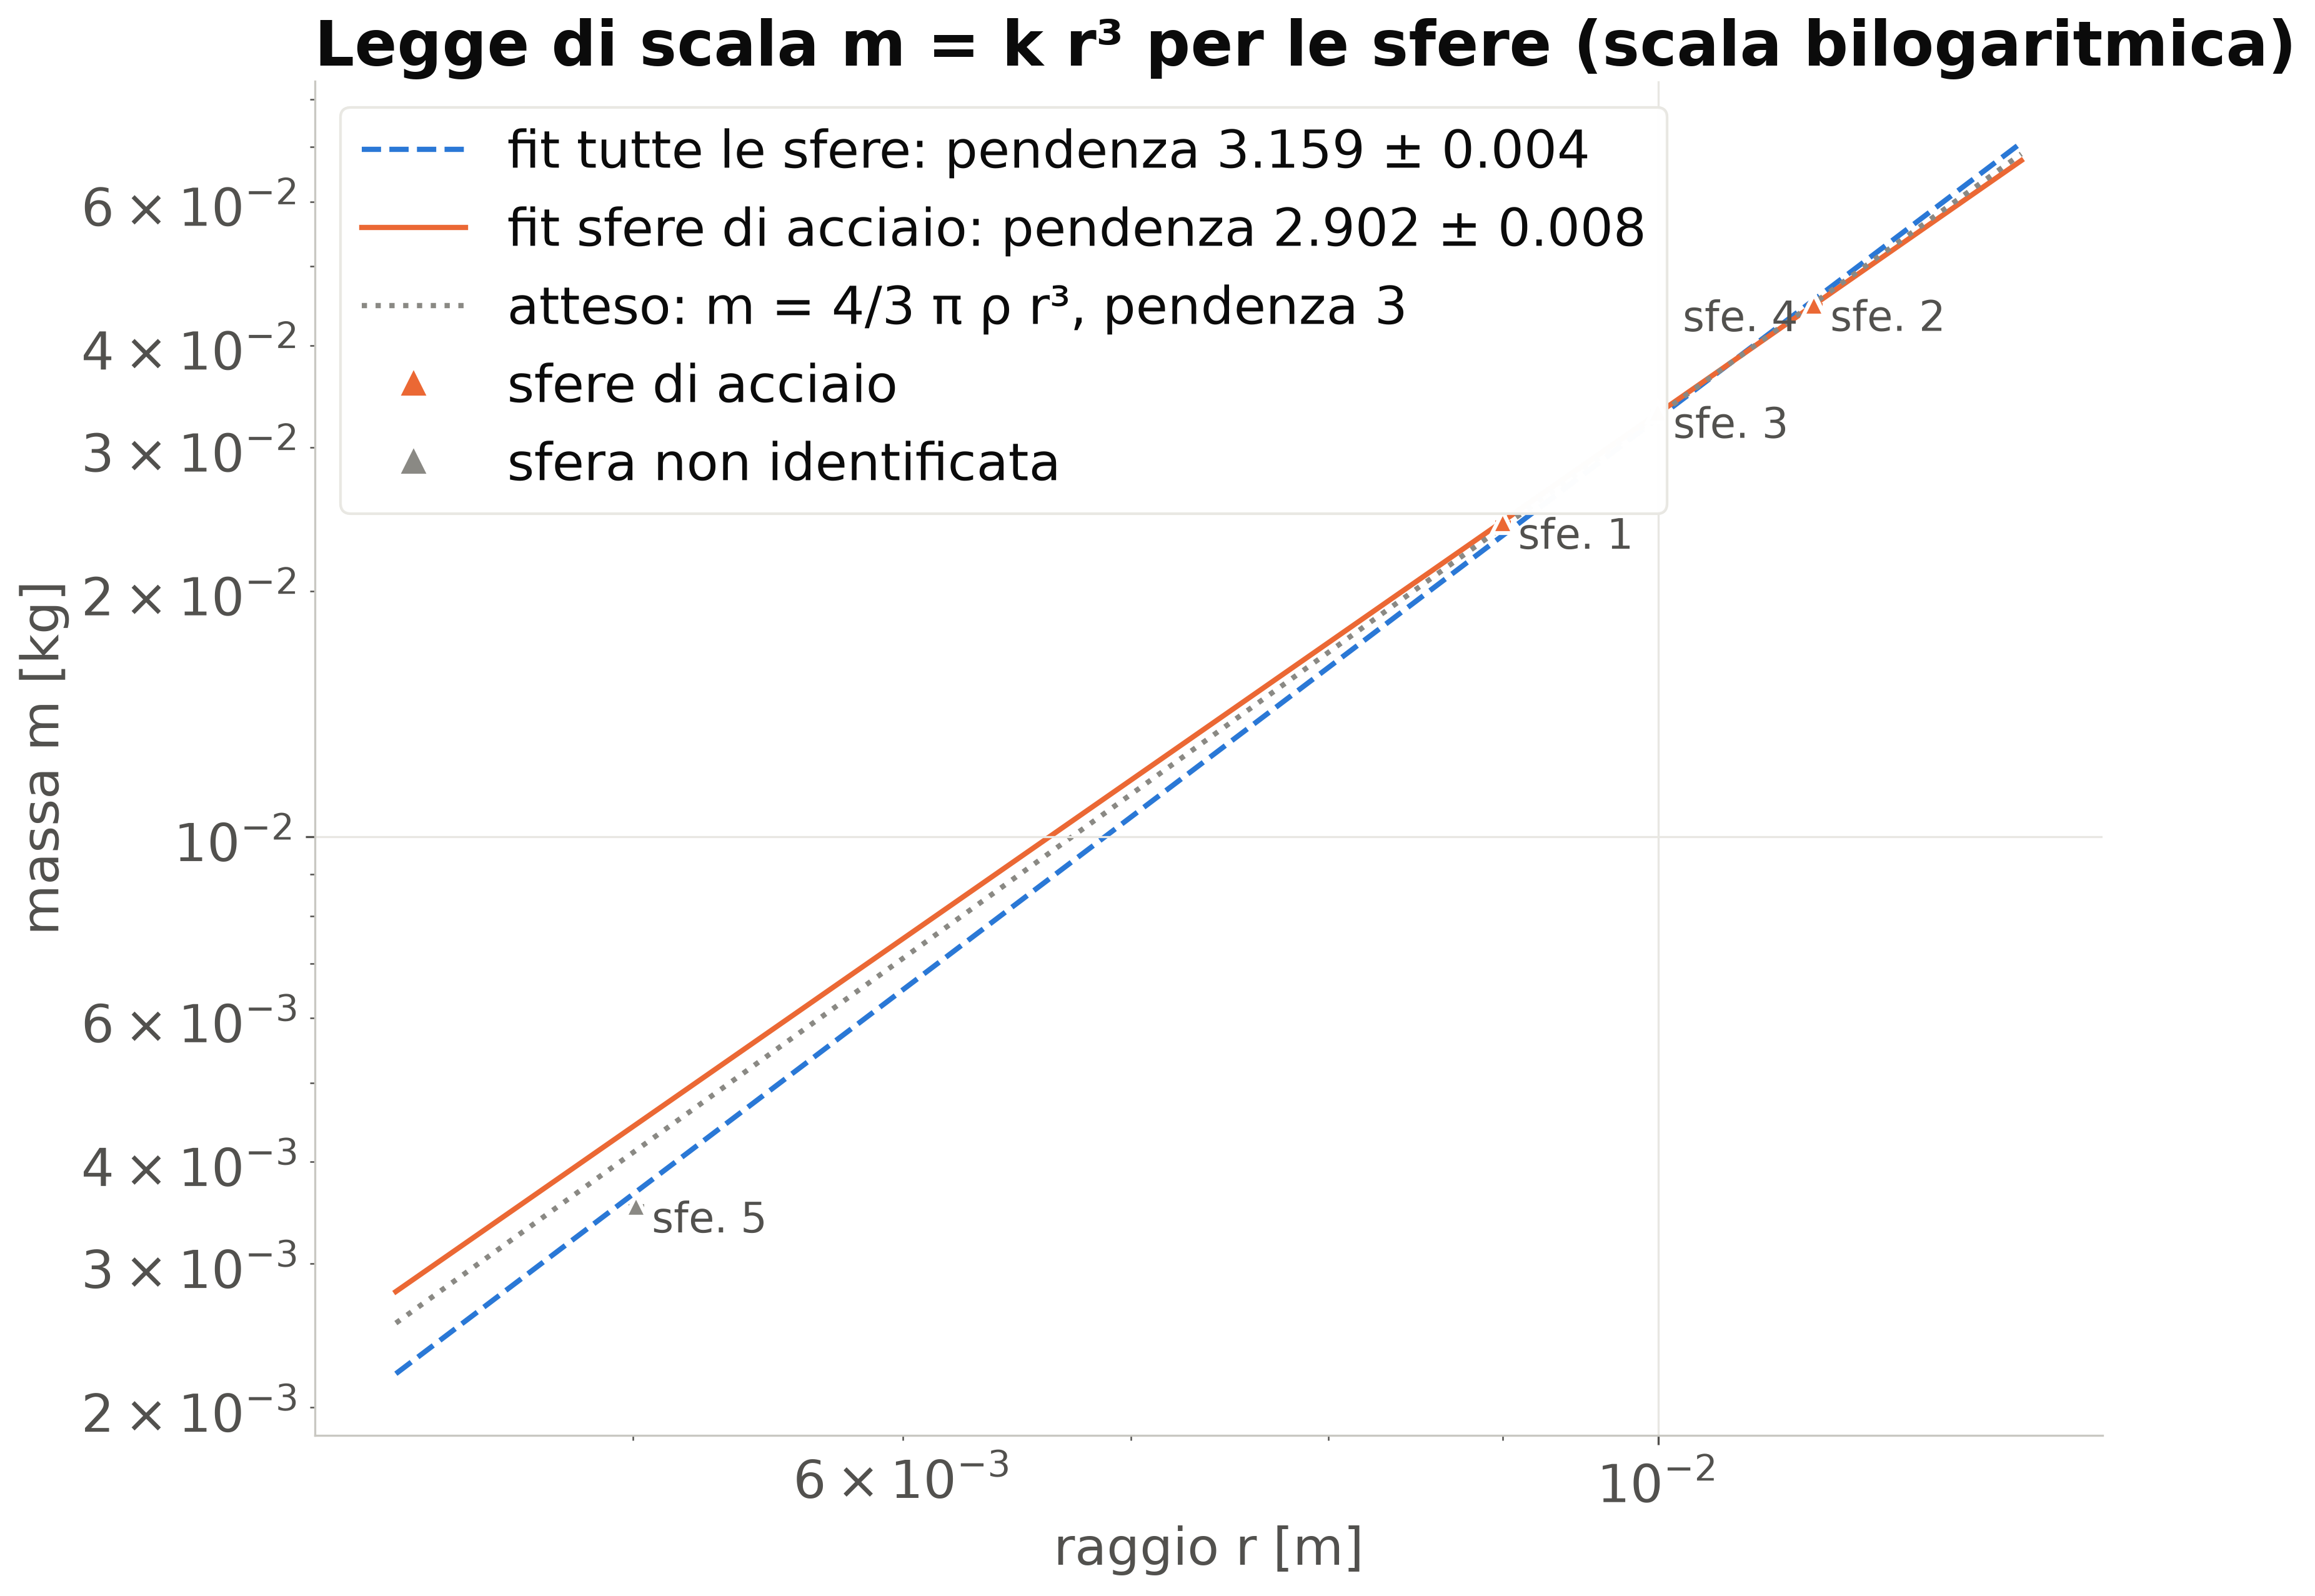
\includegraphics[width=\linewidth]{grafici/7_legge_di_scala_sfere.png}
    \caption{Massa in funzione del raggio delle sfere in scala bilogaritmica, con il fit lineare \eqref{eq:bilog}.}
    \label{fig:bilog}
\end{figure}

Dal fit (figura \ref{fig:bilog}) otteniamo $n = 2.902 \pm 0.009$. La pendenza è vicina a 3 (la differenza è del 3\%), però l'incertezza è così piccola che il valore dista circa $11\,\sigma$ da 3, quindi non è compatibile. Il motivo secondo noi è lo stesso visto per l'acciaio: le sfere più piccole (1 e 3) sono anche le più dense, quindi la massa cresce con il raggio un po' più lentamente di $r^3$. Inoltre i raggi delle quattro sfere sono abbastanza simili tra loro (da 9.0 a 11.1~mm), quindi anche una piccola differenza di densità cambia molto la pendenza.

\begin{figure}[htbp]
    \centering
    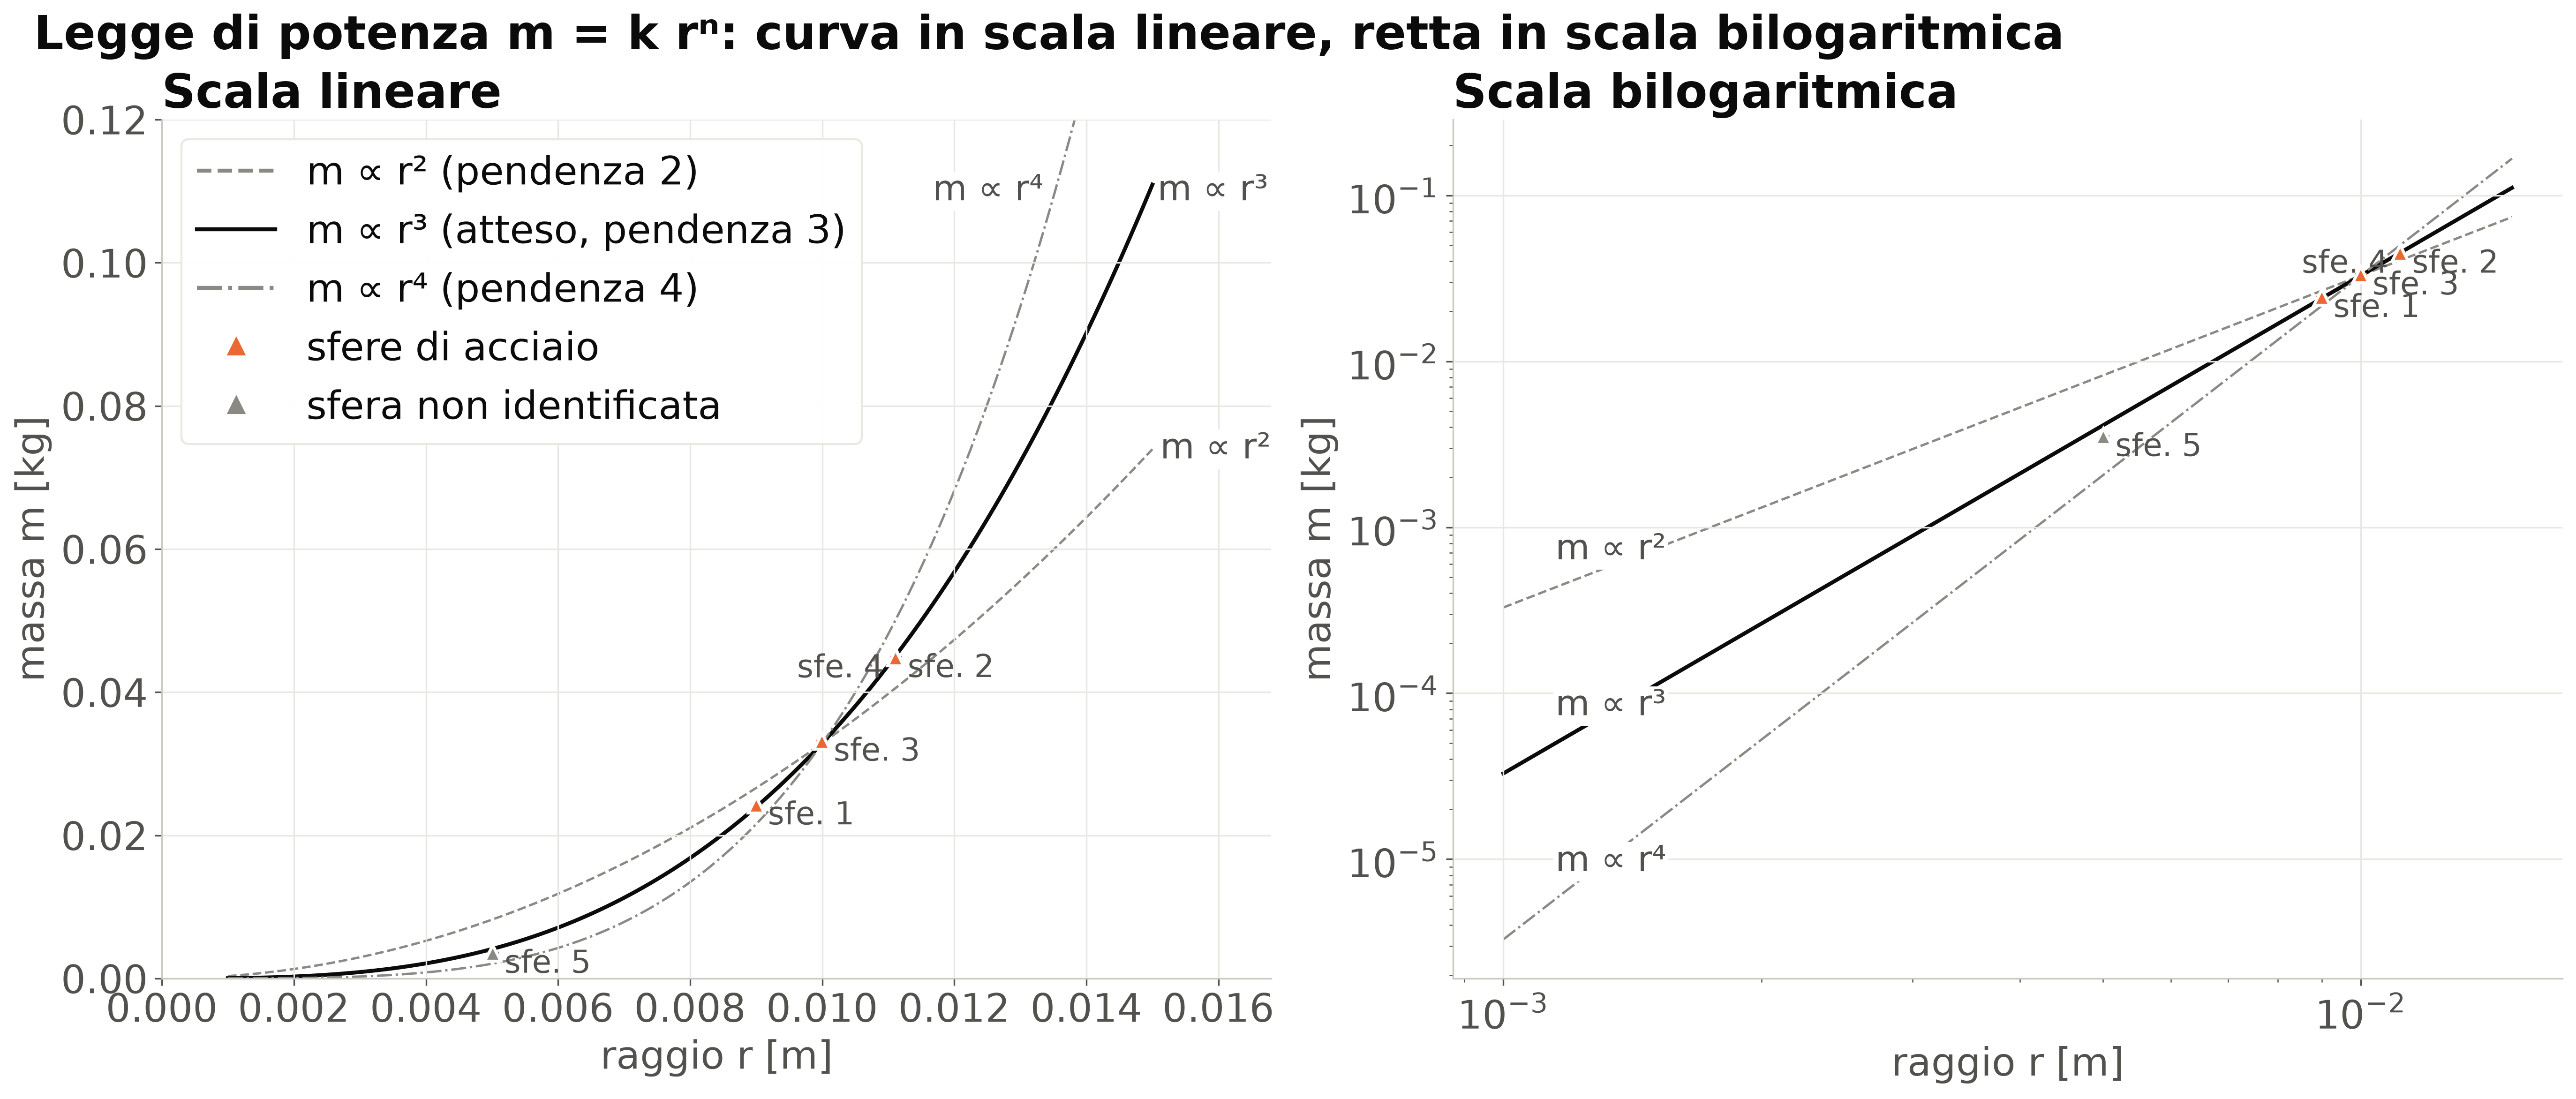
\includegraphics[width=\linewidth]{grafici/8_confronto_lineare_e_bilogaritmico.png}
    \caption{Massa in funzione del raggio delle sfere in scala lineare e in scala bilogaritmica.}
    \label{fig:confronto_scale}
\end{figure}

Infine in figura \ref{fig:confronto_scale} riportiamo gli stessi dati sia in scala lineare che in scala bilogaritmica. In scala lineare l'andamento cubico è una curva, e da lì è difficile capire l'esponente, mentre in scala bilogaritmica diventa una retta e l'esponente è semplicemente la pendenza.

\section{Conclusioni}

L'esperimento ci ha permesso di determinare le densità dei tre materiali di cui sono fatti i solidi: $2658 \pm 10$~kg/m$^3$ per l'alluminio, $8534 \pm 71$~kg/m$^3$ per l'ottone e $7675 \pm 14$~kg/m$^3$ per l'acciaio. I valori di ottone e acciaio sono dentro gli intervalli tabulati, mentre quello dell'alluminio è più basso del 2\% rispetto al valore tabulato, probabilmente perché si tratta di una lega.

Bisogna però tenere conto che per alluminio e ottone i fit sono fatti con solo due punti, quindi non possiamo verificare né che i punti siano allineati né che la retta passi per l'origine. Il cilindro 4, che era irregolare, ha poi una densità più bassa di circa il 10\% rispetto all'alluminio, probabilmente perché per un solido irregolare la formula del volume non funziona bene.

Per l'acciaio invece il fit ha dei punti fuori dalle barre d'errore e un'intercetta diversa da zero. Questo secondo noi è dovuto al fatto che i solidi in acciaio sembrano dividersi in due gruppi con densità diverse (circa 7935 e 7795~kg/m$^3$), quindi probabilmente sono fatti di due leghe diverse. Lo stesso motivo spiega anche la pendenza del grafico bilogaritmico, $n = 2.902 \pm 0.009$, che è vicina a 3 e quindi conferma che $m \propto r^3$, ma non è compatibile con 3 entro le incertezze.

\end{document}